% TexStudio Spellchecking Command
% !TeX spellcheck = de_DE_OLDSPELL

%
% Copyright Clemens H. Cap (C) 2023
% Nutzung nach Creative Commons 4.0 BY-NC-SA
%

\documentclass[a4paper]{article}%   Könnte auch book sein, aber article setzt etwas kompakter und weniger Platz verschwendend

%%% Definiere aktuelle Dokumentenvariante
%\def\mittext{}                 %% Für öffentliche Variante auskommentieren
%\def\instruktorflag{DEF}       %% Wenn definiert, dann sind auch Hinweise für Dozenten dabei. (Antworten, Namen von Referenzen)

%%
%% common.tex  Macro Datei für den IW Reader
%%

\pdfoptionpdfminorversion=7                        % Anpassen PDF Version an die PDFs 
                                                   % die im reader eingebunden werden
%%
%% Import Packages
%%
\usepackage[german]{babel}                         % Sprache und Trenntabellen auswählen
\usepackage{geometry}                              % Anpassen Seitengeometrie für Einbau
                                                   % externer DPF-Dateien
                                                   
\usepackage{fontawesome}                           % Einige nette Symbole einbinden
\usepackage{dtk-logos}                             % Wir brauchen das Bibtex Logo
\usepackage{manfnt}                                % Benötigtes Symbol einbauen
\usepackage{MnSymbol,wasysym}                      % Benötigtes Symbol einbauen

\usepackage[inline]{enumitem}                      % Anpassbare Listen aktiv, inline
\usepackage{hhline}                                % Linien für farbige Tabellen
\usepackage[table]{xcolor}                         % Farbige Zellen in Tabellen
\usepackage{adjustbox}                             % Zusatz; rotierte Tabellen
\usepackage{tabto}                                 % Bessere Tabulatoren

\usepackage{fancyhdr}                              % Sinnvolle headings auf den Seiten
\pagestyle{fancy}                                  % Heading Stil aktivieren

\usepackage{qrcode}                                % QR Code setzen

\usepackage{pdfpages}                              % Importieren von PDF Dateien

\usepackage[outputdir=build,cache=false]{minted}   % Einbinden von Code mit Highlighting
                                                   % Option für build directory
                                                   % Caching aus wegen Selbstinklusion

\usepackage{graphics}                              % Grafiken einbauen
\usepackage{pgfplots}                              % Plot Funktionen
\usetikzlibrary{automata, positioning}             % Plot Libraries einbinden
\usetikzlibrary{arrows, arrows.meta}               % Plot Libraries einbinden

\usepackage{comment}                               % Teile auskommentieren
\usepackage{todonotes}                             % Notizen für den Autor

\usepackage{titletoc}                              % Partielle Inhaltsverzeichnisse

%%
%% Optik des Layout etwas nachjustieren
%%
\parindent 0pt                                     % Kein Paragrapheneinzug
\parskip   0.25cm                                  % Paragraphenabstand
\usepackage{titlesec}                              % \titlespaceing command
\titlespacing{\paragraph}{0pt}{8pt}{16pt}          % Paragraphen kompakter
\usepackage[all]{nowidow}                          % Hurenkinder, Schusterjungen vermeiden
\setlist[enumerate]{topsep=0pt}                    % Anpassbare Listen nutzen und anpassen
\setlist[itemize]{topsep=0pt}
\setlist[enumerate]*{label={(\arabic*)}}

%%
%% Neue Seite am Ende von \part vermeiden
%%
%
% Quelle: https://tex.stackexchange.com/questions/42526/
%         how-to-remove-page-break-after-part-in-report-book
%
\makeatletter
\def\@endpart{}                                   % First, modify the \@endpart macro.
\patchcmd{\part}{\null\vfil}{}{}{}                % Third, suppress vertical whitespace 
                                                  % before "Part xx" material
\makeatother

%%
%% Einstellungen für schönere Hyperlinks
%%
\usepackage{xurl}                                  % Erlaubt bessere Trennung von URLs
\usepackage[]{hyperref}                            % Hyperlinks  
                                                   % CAVE: load hyperref AFTER titlesec
\hypersetup{
  bookmarksnumbered=true,                          % number PDF
  breaklinks=true,                                 % may break links
  colorlinks,
  linkcolor={red},                                 % internal links 
  citecolor={red}, 
  urlcolor={blue},                                 % linked urls
  filecolor={blue}                                 % urls which open local files
}

\usepackage[type={CC},                             % Setup copyright notice
            modifier={by-nc-sa}, 
            version={4.0}]{doclicense}

%%
%% Einige Convenience Abkürzungen
%%
\def\PDF{\faFilePdfO PDF}
\def\online{\faExternalLink online}
\def\tikz{Ti\textit{k}Z}

%%
%% Macro, um die totale Seitenzahl des Readers zu ermitteln
%%
%
%  \pages{ <num> }    Addiert und gibt aus
%  \pages*{ <num> }   Addiert und gibt nicht aus
%  Zähler:            totalpages
%
\newcounter{totalpages}\setcounter{totalpages}{0}  % Lokalen Zähler anlegen
\makeatletter
\def\@pages#1{\addtocounter{totalpages}{#1}}%      % Makro Seitenzahl ohne Ausgabe
\def\@@pages#1{%
  \def\one{1}%
  \def\arg{#1}%
  (#1~\ifx\one\arg{Seite}\else{Seiten}\fi)%
  \addtocounter{totalpages}{#1}}%                  % Makro Seitenzahl MIT Ausgabe
\def\pages{\@ifstar\@pages\@@pages}%
\makeatother

%%
%% Referenzen über mehr als einen LaTeX-Lauf merken
%%
%
%  Bsp: Wert von totalpages am Ende des Dokuments in totalPageNumber speichern     
%       \storereference{totalPageNumber}{\thetotalpages}
%
%       Wert von totalPageNumber an anderer Stelle nutzen                    
%       \crtrefnumber{totalPageNumber}
%
\usepackage{crossreftools}
\crtrefundefinedtext{0}                            % Undefinierte Referenzen sind 0
\newcommand{\storeReference}[2]{\crtcrossreflabel*{#2}[#1]}


%%
%% \glabel definiert einen globalen label, der in \currentLabel gespeichert wird
%% Benötigt für die backlinks, wo eine Aufgabe etc benutzt wurde
%%
\def\glabel#1{\label{#1}\hypertarget{#1}{}\gdef\currentLabel{#1}}

%%
%% LATEXTRAINING
%%
%   \latexaufgabe  Setzt die Titel-Zeile für eine Aufgabe
%   \latexaufgabe{ <Bezeichnung-der-Aufgabe> }{ <label-zum-referenzieren-der-aufgabe> }
%
%   \uselatexaufgabe  Verweist auf eine Aufgabe im Text
%   \uselatexaufgabe{ <label-zum-referenzieren-der-aufgabe> }
%   Bsp: Wir bearbeiten \useaufgabe{ <label-zum-referenzieren-der-aufgabe> }
%
\def\latexaufgabe#1#2{%
  \stepcounter{latexaufgabencounter}%
  \subsection*{\phantomsection\relax \hypertarget{#2}{}#1%
     \ifdefined\instruktorflag{\hfill\color{gray}#2}\fi}%      
   \label{lt\thelatexaufgabencounter}%
  %   Referenznamen nur in Dozentenversion zeigen
  \addcontentsline{toc}{subsection}{#1}%
  \storeReference{#2}{#1}%    Speichere Bezeichnung unter dem label
}

\def\uselatexaufgabe#1{\hyperlink{#1}{\crtrefnumber{#1}}}

\newcounter{latexaufgabencounter}


%%
%% AUFGABEN
%%
%   \aufgabe  Setzt die Titel-Zeile für eine Aufgabe
%   \aufgabe{ <Bezeichnung-der-Aufgabe> }{ <label-zum-referenzieren-der-aufgabe> }
%
%   \useaufgabe  Verweist auf eine Aufgabe im Text
%   \useaufgabe{ <label-zum-referenzieren-der-aufgabe> }
%   Bsp: Wir bearbeiten \useaufgabe{ <label-zum-referenzieren-der-aufgabe> }
%
\def\aufgabe#1#2{%
  \stepcounter{aufgabencounter}%
  \hypertarget{#2}{}%        Target für \useaufgabe setzen
  \label{#2}% 
  \subsection*{\phantomsection\relax Aufgabe \theaufgabencounter:~#1%
     \ifdefined\instruktorflag{\hfill\color{gray}#2}\fi}%       
  % Referenznamen nur in Dozentenversion zeigen
  \addcontentsline{toc}{subsection}{Aufgabe \theaufgabencounter:~#1}%
  \storeReference{#2}{Aufgabe \theaufgabencounter:~#1}%     Speichere Mapping von 
                                         %  Aufgaben-Label zu Aufgabenbezeichnung
  \storeReference{AU#2}{\theaufgabencounter}%  Maps label to number
  \textbf{Behandelt:} In \nameref{\crtrefnumber{Label#2}}.
}
\def\useaufgabe#1{\hyperlink{#1}{\crtrefnumber{#1}}%
  \storeReference{Label#1}{\currentLabel}% Mapping von "Label" gefolgt 
  %         von Aufgaben-Label zu Label der Unit wo es behandelt wird
  \ifdefined\instruktorflag{\hfill\color{gray}#1} \fi%
}
\newcounter{aufgabencounter}

\def\sa#1{\hyperlink{#1}{\bf\crtrefnumber{AU#1}}}%  given a label provides a link to the aufgabe


%%
%% VORFÜHRUNGEN
%%
%
%  \demo  Setzt die 
%  \demo{ <Bezeichnung-der-Vorführung> }{ <label-zum-referenzieren-der-Vorführung> }
%  \usedemo{ <label-zum-referenzieren-der-Vorführung> }
%
\def\demo#1#2{
  \stepcounter{democounter}%
  \hypertarget{#2}{}%        Target für \usedemo setzen
  \subsection*{\phantomsection\relax Vorführung \thedemocounter:~#1%
    \ifdefined\instruktorflag{\hfill\color{gray}#2}\fi}%
  \label{vor\thedemocounter}%  vor<number> ist der label space der Vorführungen
  %  Referenznamen nur in Dozentenversion zeigen
  \addcontentsline{toc}{subsection}{Vorführung \thedemocounter:~#1}%
  \storeReference{#2}{Vorführung \thedemocounter:~#1}  
}
\def\usedemo#1{\hyperlink{#1}{\crtrefnumber{#1}}}
\newcounter{democounter}


%%
%% UNITS
%%
%   #1  Name to be written    
%   #2 Label used for referencing (needed in case of \LaTeX in title)
\newcounter{unitcounter}\setcounter{unitcounter}{0}%           Zähler für Units
\def\unit#1#2{%                                                Header für Leseeinheit setzen
  \clearpage%
  \stepcounter{unitcounter}%
  \setcounter{header}{1}%                                      Neue Nummerierung
  \lhead{Reader}%                                              Linke Header in Unit
  \rhead{Einheit \theunitcounter: #1}%                         Rechter Header in Unit
  \hypertarget{#2}{}%                                          Target setzen zur Unit
  \storeReference{#2}{Reader Einheit \theunitcounter:~#1}%
  \storeReference{Num#2}{\theunitcounter}%
  \section*{\phantomsection\relax Einheit \theunitcounter: #1%
    \ifdefined\instruktorflag{\hfill\color{gray}#2}\fi}%
    \label{unit\theunitcounter}%
  \addcontentsline{toc}{section}{Einheit \theunitcounter:~#1}%
  \gdef\unitName{#1}
}

\def\useunit#1{\hyperlink{#1}{\crtrefnumber{#1}}}% Referenziere ganze Reader Unit über Namen.

\def\uu#1{\hyperref[\crtrefnumber{#1}]{#1}}%  referenziere reader unit über namnen, zeige nummer

\newcounter{header}\setcounter{header}{1}%    Subzähler für einzelne Elemente in Einheiten

%%
%% Zur Formatierung jener Teile im Reader, die auf derselben Ebene wie die \units sind
%% die aber selber nicht Einheiten sind, und sich daher anders verhalten müssen (Links etc)
%% Bsp: Vorwort Nachwort
%%
\def\mysection#1{
  \clearpage%
  \lhead{Reader}%
  \rhead{#1}%
  \phantomsection%   \section* setzte keine hypertargets
  \section*{#1}%
  \addcontentsline{toc}{section}{#1}%
}

%%
%% Im Footer rechts überall einen Link zurück zum Inhaltsverzeichnis setzen
%%
\rfoot{\hyperlink{Inhaltsverzeichnis}{\faListOl}}% 

%%
%% Pagestlye für den Reader / PDF Import setzen
%%
%  Quelle in den Footer schreiben.
%
\fancypagestyle{pdfpages}{%                       Page style für Reader definieren
  \renewcommand{\headrulewidth}{0pt}%             Keine Trennlinie im Header, denn wir haben 
%                                                 einen Rahmen in variabler Länge je nach
%                                                 Größe der importierten Seite
  \fancyfoot[L]{\footnotesize\pdfpagesfooter}
  \fancyfoot[C]{}%                                Zentrierter Footer wäre die Seitenzahl, 
  %                                               die wir im Reader nicht brauchen
  \fancyfoot[R]{\hyperlink{Inhaltsverzeichnis}{\faListOl}\hspace*{-1cm}}%
}

\newcommand*\pdfpagesfooter{}

\newcommand{\setlayout}[1]{%               Macro um Page Style (footer) auf der 
%                                          spezifischen Seite des PDF Include zu setzen
  \thispagestyle{pdfpages}%                Auf pdfpages page style umschalten
  \gdef\pdfpagesfooter{#1}%                Parameter in globaler Variablen speichern
}


%%
%% Pagestyle für den Anhang definieren
%%
\fancypagestyle{anhang}{
  \fancyhead[L]{}
  \fancyhead[C]{Anhang}%                                
  \fancyhead[R]{}%
}





%%
%% READER-INHALT
%%
%
%  \add         Definieren ein Inhaltselement im Reader
%    #1 Header Text für den Inhalt, dient auch als Label für Verweise    
%       CAVE:   Darf keine Sonderzeichen enthalten wegen Nutzung als Label
%    #2 Text der den Inhalt beschreibt
%    #3 Filename des Inhalts, inklusive Pfad                    oder leer {}
%    #4 Ein vollständiger Link is web in der Form \href{}{}     oder leer {}
%
\makeatletter
\newwrite\appendFile
\immediate\openout\appendFile=appendFiles.lst
\def\add#1#2#3#4{%
  \hypertarget{Kom:#1}{}%                        Target für das Kommentar setzen
  \textbf{\S \theunitcounter.\theheader:~#1} #2%  
  \def\argFile{#3}%                              Parameter in Variable speichern 
  %                                              nötig für Vergleich mit leerem Macro
  \ifx\argFile\empty\else%                       Wenn File vorhanden, 
    \relax\space\hyperlink{Ank:#1}{\PDF}\fi%     Link setzen auf Ankündigungsseite
  \def\argu{#4}%
  \ifx\argu\empty\else\relax\space\argu\fi%
  \ifx\argFile\empty\else%                       Wenn File vorhanden, 
    \write\appendFile{%                          Ankündigungsseite;  File inkludieren
      \unexpanded{\hypertarget}{#3}{}%
      \unexpanded{\hypertarget}{Ank:#1}{}%       Target für die Ankündigungsseite
      \unexpanded{\rhead{}\lhead{}}%             Header der Ankündigungsseite löschen
      \unexpanded{\chead}{\footnotesize\textbf{Einheit \theunitcounter:~\unitName}% 
        \hfill \textbf{Text:}~#1}%               Header Ankündigungsseite  
      \unexpanded{\phantomsection}%
      \unexpanded{\addcontentsline}{toc}{section}{#1}%
      \unexpanded{\large}%
      \unexpanded{\renewcommand\baselinestretch{1.2}}%
      \unexpanded{\topskip0pt\vspace*{\fill}}%
      \unexpanded{\textbf}%
      {#1} \\[6pt]%
      #2   \\[6pt]%
      #4
      \unexpanded{\vspace*{\fill}}%
      \unexpanded{\normalsize}%
      \ifdefined\mittext
        \unexpanded{\includepdf[pages=-, 
                                pagecommand=\setlayout{\textbf{Quelle:}~#2}, 
                                width=\textwidth,
                                height=\textheight,
                                keepaspectratio,
                                frame]}{#3}%
      \else\par
         Den Text finden Sie aus urheberrechtlichen Gründen nur 
         in der eingeschränkten Variante dieses Dokuments oder
         online unter der Verantwortung der entsprechend verlinkten Site.
         \vfill\pagebreak
      \fi
     %
      }%
  \fi%
  \stepcounter{header}%
}
\makeatother

\usepackage{csquotes}                         % Quotes; Paket möglichst spät laden

\ifdefined\instruktorflag%                      Wenn instruktorflag gesetzt
  \usepackage[firstpageonly=true]{draftwatermark}% Watermark auf Frontseite zur Warnung
\fi
%                %% Style File für den Reader einlesen

\title{Informatik und Wissenschaft \\[12pt] \normalsize Arbeitsmaterialien, Aufgabensammlung und Reader}
\author{Clemens H. Cap}
\date{\today, Version 1.4}

\begin{document}

\maketitle

\ifdefined\instruktorflag\SetWatermarkText{Interne Version}\SetWatermarkScale{3}\fi

\begin{quote}

\textbf{Hinweis:} Aus urheberrechtlichen Gründen gibt es dieses Dokument in zwei Varianten.
Die \textit{öffentliche Variante} enthält nur die Referenzen auf die Texte des Readers.
Die \textit{eingeschränkte Variante} wendet sich an die Teilnehmer meiner entsprechenden Lehrveranstaltung
und gibt im Teil 3 (Reader) auch die zitierten Texte nach \href{https://dejure.org/gesetze/UrhG/60a.html}{\S 60a UrhG}
wieder; sie ist nur hochschulintern zugänglich.

\ifdefined\mittext\textbf{Dieses Exemplar ist die eingeschränkte Variante.
Sie darf daher weder weitergegeben noch öffentlich
zugänglich gemacht werden.}
\else\textbf{Dieses Exemplar ist die öffentliche Variante.}\fi

\vfill

\textbf{Copyright in den Teilen 1 und 2:}  Clemens H. Cap, \copyright 2023.
\doclicenseThis

\textbf{Copyright im Teil 3:} Es gilt das Copyright der jeweiligen Rechteinhaber.

\vfill

\begin{tabular}[]{@{}c@{}}  % Doppelte @{} um komplett bündig zu setzen
\qrcode[hyperlink,height=2in]{https://iuk.one} \\  \\[2pt] 
\href{https://iuk.one}{Verteilung auf https://iuk.one}
\end{tabular}\hfill\begin{tabular}[]{@{}c@{}}
\qrcode[hyperlink,height=2in]{https://github.com/clecap/vorlesung-informatik-und-wissenschaft/settings} \\ \\[2pt]
\href{https://github.com/clecap/vorlesung-informatik-und-wissenschaft}{Quellen des Dokuments} \\
\href{https://github.com/clecap/vorlesung-informatik-und-wissenschaft}{auf https://github.com/clecap/}
\end{tabular}

\vfill

Hinweise auf Fehler im Dokument bitte im Repository \url{https://github.com/clecap/vorlesung-informatik-und-wissenschaft}
als \href{https://github.com/clecap/vorlesung-informatik-und-wissenschaft/issues}{\textit{issue}} einpflegen.

\end{quote}



\subsection*{Versionsgeschichte}

\textbf{Version 1.4}
\begin{itemize}
\item Anpassung des Wording Präsenzübung: Es gibt nur eine Form von Übungen.
\item Anpassung der Zeitpläne an 2023.
\item Behebung kleiner Schreib- und Verständnisfehler.
\item Einfügen von Hinweisen und Beiträgen zu ChatGPT.
\item Kleine inhaltliche Anpassungen.
\item Anpassungen in der Aufgabenstellung der Hausarbeit.
\item Entfernung der Teile für die IWG Vorlesung des 7. Semesters.
\item Verbesserung der Numerierung, Strukturierung und Gliederung.
\item Anpassung einzelner Aufgabenstellungen.
\item Veröffentlichung der Quellen auf Github.
\item Anpassung des Copyright für eigene Teile an Creative Commons.
\end{itemize}

\vfill

\textbf{Danksagung}

Ich danke meinem Mitarbeiter \textsc{Richard Dabels} für viele Hinweise und Vorschläge, die
zur Verbesserung dieses Dokuments geführt haben.


\clearpage

\vspace*{\fill}

{\raggedright
\begin{quote}
Alle Hindernisse und Schwierigkeiten sind Stufen,\\
auf denen wir in die Höhe steigen.\\[12pt]
\hfill \textsc{Friedrich Nietzsche}\footnote{\textsc{Nietzsche} zugeschrieben nach: H. Brosche: Warum es nicht so schlimm ist, in der Schule
schlecht zu sein. Kösel-Verlag, 2009. Siehe aber auch: \url{https://falschzitate.blogspot.com/2019/05/hindernisse-und-schwierigkeiten-sind.html}.}, Deutscher Philosoph
\end{quote}
}


{\raggedright
\begin{quote}
Bildung ist letztlich viel mehr \\ als einzelne Fakten auswendig zu lernen.\\
Was am wichtigsten ist: \\ Lernen selber zu denken, \\ lernen zu argumentieren und \\ lernen wie man am besten lernt.\footnote{Quelle: \url{https://de.wikipedia.org/wiki/Vitalik\_Buterin}.}\\[12pt]
\hfill\textsc{Vitalik Buterin}, Mitbegründer von Ethereum
\end{quote}
}

\clearpage


\clearpage

\pagebreak\hypertarget{Inhaltsverzeichnis}{}
\tableofcontents


\clearpage


\part{Übersicht und Aufgabensammlung}

\startcontents[part1]
\printcontents[part1]{}{1}[1]{}

\clearpage%  Force start on next page and thereby improve positioning of PDF bookmark target; due to my use of article style


\section{Ziel und Inhalte}\label{ZieleUndInhalte}

\paragraph{Ziel:} Die Lehrveranstaltung \enquote{Informatik und Wissenschaft} (IW) 
führt im 2. Semester des Bachelor-Studiums in das wissenschaftliche Arbeiten in Informatik ein.


\paragraph{Inhalte:} In der Veranstaltung werden die folgenden Themenfelder behandelt:
\begin{enumerate}
\item \textbf{Lernen:} \hfill Strategien für ein leichteres und effizienteres Lernen.
\item \textbf{Wissenschaft:} \hfill Einführung in wissenschaftliches Arbeiten und Methoden.
\item \textbf{Organisieren:} \hfill Zeit- und Selbstmanagement, Strategien zum Meistern des Studiums.
\item \textbf{Lesen:} \hfill Techniken des schnellen und des auswertenden Lesens.
\item \textbf{Literatur:} \hfill Arbeiten mit wissenschaftlicher Literatur.
\item \textbf{Schreiben:} \hfill Wissenschaftlicher Schreibstil.
\item \textbf{Vortragen:} \hfill Gestaltung eines Vortrags.
\item \textbf{Paper:} \hfill Praktische Übung anhand eines kurzen Papiers.
\item \textbf{\LaTeX:} \hfill Einführung in den Textsatz für Ingenieur- und Naturwissenschaften.
\end{enumerate}


\paragraph{Fortsetzung:} Im 7. Semester schließt die Lehrveranstaltung \enquote{Informatik, Wissenschaft und Gesellschaft} (IWG) an.
Sie vertieft einige Inhalte, geht auf die besondere gesellschaftliche Verantwortung des Informatikers ein,
bespricht das Verhältnis zwischen Wissenschaft und Gesellschaft und bereitet auf die Bachelorarbeit als 
selbständige wissenschaftliche Arbeit vor.

\clearpage


\clearpage
\section{Organisation und Ablauf}\label{OrganisationUndAblauf}

\subsection{Elemente}

Die Lehrveranstaltung umfaßt die folgenden Elemente:

Die \hyperref[Digitalvorlesung]{\textbf{Digitalvorlesung}} besteht aus aufgenommenen Vorlesungen (Video/Audio-Strom sowie
Unterlagen in PDF-Form). Sie dient der ersten Wissensvermittlung.
Sie wird von Ihnen \textit{nach eigenem Zeitplan selb\-ständig} angesehen und individuell oder in selbstorganisierten Gruppen erarbeitet.
Die dabei entstandenen Fragen bringen Sie in die Präsenzvorlesung mit.

Die \hyperref[Prsenzvorlesung]{\textbf{Präsenzvorlesung}} arbeitet nach dem Modell des \textit{inverted} oder 
\textit{flipped classroom}\footnote{Mehr dazu siehe \url{https://www.e-teaching.org/lehrszenarien/vorlesung/inverted_classroom}.}
Dieses setzt eine Beschäftigung mit den Materialien
der Digitalvorlesung und des Readers (s. unten)
als Vorbereitung  voraus. 
Die Veranstaltung wiederholt und diskutiert das erworbene Wissen.
Dabei können entstandene Fragen geklärt werden.
In der gemeinsamen Anwendung des Wissens auf Beispiele
sollen Grenzfälle ausgelotet werden und die eigene Modellbildung kann auf
den Prüfstand gestellt werden.
Da der Stofferwerb teilweise bereits vor der Präsenzvorlesung erfolgt ist, kann dabei eine
Kontrolle und ein Nachjustieren der erworbenen Kenntnisse erfolgen.

Die \hyperref[Ubung]{\textbf{Übung}} setzt eine \textit{vorangehende Bearbeitung} von Übungsaufgaben voraus.
Sie dient der praktischen Einübung von Standardverfahren des wissenschaftlichen Arbeitens; sie bietet
Raum für weitere Diskussionen und ergänzende Sichtweisen.

Die \hyperref[Hausarbeit]{\textbf{Hausarbeit}} ist eine \textit{eigenständige Arbeitsprobe} über das erworbene Wissen. Sie schließt diese Lehrveranstaltung
als \textit{(einzige) Prüfungsleistung} ab und wird mit den Attributen \enquote{bestanden} oder \enquote{nicht bestanden} bewertet.

\textit{Eigenständig} bedeutet bei der Hausarbeit, daß Sie die Texte selber entwickeln und sich diese nicht von Programmen wie ChatGPT schreiben lassen.
Plagiate -- das sollte in einer Lehrveranstaltung über wissenschaftliches Arbeiten eigentlich selbstverständlich sein --
führen zu einer negativen Bewertung der Hausarbeit und werden nach den Regeln der Studienordnungen sanktioniert.

Betrachten Sie diese Lehrveranstaltung und die begleitenden Aufgaben als Fitness-Training für Ihr Gehirn: Machen Sie die
Aufgaben selber und lernen Sie in den Übungen und in den Präsenzvorlesungen dabei aus Ihren Fehlern!
Auch im Fitness-Center strampeln Sie am Standfahrrad selber, um Kreislauf und Muskeln zu trainieren, und 
schließen das Fahrrad nicht an einen Elektromotor an. 

Die \hyperref[auf]{\textbf{Aufgaben}} umfassen Fragestellungen, die zu einer intensiveren praktischen
Beschäftigung mit dem Stoff anregen. Jede Aufgabe
wird entweder in einer Präsenzvorlesung oder in einer Übung mit den Teilnehmern behandelt.

Drei \hyperref[vor]{\textbf{Vorführungen}} umfassen Demonstrationen, die in den Übungen gemeinsamen mit den
Teilnehmern durchgeführt werden. Zum Nachvollziehen empfiehlt sich die Mitnahme eines
Laptop in die Übung.

Der \hyperref[Reader1]{\textbf{Reader}} besteht aus einer kommentierten Auswahl von Texten. Er dient der Ergänzung der
Digitalvorlesung. Er soll zu einer weitergehenden Befassung mit dem Stoff anregen und Ausgangspunkt für
Fragen und Diskussionen in der Präsenzvorlesung und in der Übung sein.
Einzelne Elemente der Lehrveranstaltung verweisen daher auf Teile des Readers.

\pagebreak



\subsection{Struktur}


Die Übungen bestehen aus einem durchgehenden \LaTeX-Kurs, drei praktischen Vorführungen
und drei Terminen zur Besprechung der von Ihnen dazu vorbereiteten
Fragen betreffend der drei Teile der Hausarbeit.


% Definition von Farbzellen
\def\blu{\cellcolor{blue!25}}
\def\red{\cellcolor{red!25}}
\def\yel{\cellcolor{yellow!25}}
\def\gre{\cellcolor{green!25}}


\def\VL#1{\hyperref[VLIW#1]{\textbf{VL #1}}}
\def\UE#1{\hyperref[UEIW#1]{\textbf{UE #1}}}

\def\H#1{\hyperref[H#1]{\textbf{#1}}}

\def\V#1{\hyperref[vor#1]{\textbf{#1}}}

\def\LT#1{\hyperref[lt#1]{\textbf{#1}}}
\def\U#1{\hyperref[unit#1]{\textbf{#1}}}


% https://tex.stackexchange.com/questions/32683/rotated-column-titles-in-tabular
% Schiefen Tabellenheader setzen
\newcolumntype{R}[2]{%
  >{\adjustbox{angle=#1,lap=\width-(#2)}\bgroup}%
  l%
  <{\egroup}%
}
\newcommand*\rot{\multicolumn{1}{R{45}{1em}}}% no optional argument here, please!

{\setlength{\arrayrulewidth}{1.0pt}% Helps to prevent line color from being overwritten by cell color 
\setlength\extrarowheight{4pt}
\begin{table}[h]
\begin{center}
\begin{tabular}[]{@{}|l|c|c|c|c|c|c|c|c|c|c|c|}
 \multicolumn{1}{c}{} &\rot{\bf \hyperref[latex]{\LaTeX\ Training}} &  \rot{\bf \hyperref[vor]{Vorführung}} & \rot{\bf \hyperref[Hausarbeit]{Hausarbeit}} & \rot{\bf Lernen}  & \rot{\bf Wissenschaft}&\rot{\bf Organisieren}& \rot{\bf Lesen} &\rot{\bf Literatur}& \rot{\bf Schreiben} & \rot{\bf Vortragen} & \rot{\bf Paper}   \\[1pt] \hline
\multicolumn{12}{c}{\bf\large Vorlesungen} \\ \hline
\VL1 & \red &  && \blu & \blu                  &                      &                    &                      &              &       &  \\
\VL2 &  &  &&      &                       &                 &                    &    \blu                   &              &       &     \\
\VL3 &  &  &&      &                       &                      &                    &    \blu                    &              &      &    \\
\VL4 &  &  &&      &   \blu                &                      &                    &                    &      \blu        &      &     \\
\VL5 &  &  &&      &   \blu                &                      &                    &                        &          &      &   \\
\VL6 &  &  & \gre \H3 &      &  \blu                 &                      &                    &                        &              &   & \blu \\ \hline 
\multicolumn{12}{c}{\bf\large Übungen} \\ \hline
\UE1 & \red \LT1   &   \yel \V1   &            &  & \blu                  &                      &                    &                      &              &       &  \\
\UE2 & \red \LT2   &   \yel \V2   &\gre \H1    &  &                       & \blu                 &                    &     \blu             &              &       &     \\
\UE3 & \red \LT3   &   \yel \V3   &            &  &                       &                      &   \blu             &     \blu             &              &       &   \\
\UE4 & \red \LT4   &            &              &  &                       &                      &                    &                       &   \blu           &       &    \\
\UE5 & \red \LT5   &            & \gre \H2     &  &                       &                      &                    &                        &        &  \blu      &  \\
\UE6 & \red \LT6   &            & \gre \H3     &  &  \blu                 &                      &                    &                        &              &   & \blu \\ \hline
\end{tabular}
\end{center}
\caption[Struktur der Übungen]{\textbf{Übersicht über die Struktur} der Vorlesungen und Übungen: In welchen Stunden behandeln wir welche Themenfelder?}
\label{tab:uebungsstoff}
\end{table}
}


\clearpage

\subsection{Was ist vorzubereiten?}

Die einzelnen Elemente der Lehrveranstaltung sind miteinander verzahnt.
Damit leichter ersichtlich wird, auf wann was vorbereitet werden soll, habe ich
die folgenden beiden Tabellen erstellt:


{\setlength{\arrayrulewidth}{1.0pt}% Helps to prevent line color from being overwritten by cell color 
\begin{table}[h]
\begin{center}
\begin{tabular}[]{@{}l|c|c|c|c|c|c|c|}
                                & \rot{\bf \hyperref[auf]{Aufgaben}} &  \rot{\bf \hyperref[Reader1]{Reader}} &\rot{\bf \hyperref[DV]{DigitalVL}} \\[1pt] \hline
\VL1 &                    & \yel  \U1, \U2, \U3&        \\
\VL2 &  \sa{ZitateVerbessern}                  & \yel \U6  &  \gre \hyperref[DV]{\bf DV1}      \\
\VL3 &  \sa{LiteraturBewerten}, \sa{Predator}                 &  \yel \U6  & \gre  \hyperref[DV]{\bf DV1}      \\
\VL4 &  \sa{EmpirischeDaten}, \sa{Zeitmessung}, \sa{sema}, \sa{Interpol}, \sa{Skinterpol}, \sa{Notensystem}              & \yel \U7, \U8  &  \gre \hyperref[DV]{\bf DV2}, \hyperref[DV]{\bf DV3}       \\
\VL5 &   \sa{Datenbereinigung}, \sa{Sonne},  \sa{GenauesFormulieren}, \sa{Experiment}, \sa{KognitiveVerzerrungen}                 & \yel \U{10}  &    \gre    \hyperref[DV]{\bf DV4}    \\
\VL6 & \sa{Anforderungen},  \sa{Papier}            &  \yel \U3    &  \gre \hyperref[DV]{\bf DV5} \\ \hline
\end{tabular}
\end{center}
\caption[Vorbereitung auf die Präsenzvorlesungen]{\textbf{Vorbereitung auf die Präsenzvorlesungen:} Bis wann ist was vorzubereiten? 
Welche Aufgaben sind vorzubereiten?
Welche Einheiten im Reader sollen bis wann gelesen werden? 
Welche Digitalvorlesungen sollen wann angesehen werden?
Bei \VL1 handelt es sich um eine \textit{Nach}bereitung, in allen anderen Fällen um eine \textit{Vor}bereitung.
}
\label{tab:preparevl}
\end{table}
}



{\setlength{\arrayrulewidth}{1.0pt}% Helps to prevent line color from being overwritten by cell color 
\begin{table}[h]
\begin{center}
\begin{tabular}[]{@{}l|c|c|c|c|c|c|c|}
                                &\rot{\bf \hyperref[latex]{\LaTeX\ Training}} &  \rot{\bf \hyperref[auf]{Aufgaben}} & \rot{\bf \hyperref[Reader1]{Reader}} &\rot{\bf \hyperref[DV]{DigitalVL}} \\[1pt] \hline
\hyperref[UEIW1]{\textbf{UE 1}} & \red \LT1                   &                              & \yel \U1, \U3&        \\
\hyperref[UEIW2]{\textbf{UE 2}} & \red \LT2                   &                        & \yel \U1, \U4  &  \gre \hyperref[DV]{\bf DV1}      \\
\hyperref[UEIW3]{\textbf{UE 3}} & \red \LT3                   &   \sa{LiteraturSuche}, \sa{Suchen}                    & \yel \U1, \U5  & \gre  \hyperref[DV]{\bf DV1}      \\
\hyperref[UEIW4]{\textbf{UE 4}} & \red \LT4                   &   \sa{FormVerbessern}                      & \yel \U1, \U7, \U8  &  \gre \hyperref[DV]{\bf DV3}      \\
\hyperref[UEIW5]{\textbf{UE 5}} & \red \LT5                   &                  & \yel \U1, \U9  &            \\
\hyperref[UEIW6]{\textbf{UE 6}} & \red \LT6                   &                 & \yel  \U1    &  \gre \hyperref[DV]{\bf DV5} \\ \hline
\end{tabular}
\end{center}
\caption[Vorbereitung auf die Übungen]{\textbf{Vorbereitung auf die Übungen:}
Welche \LaTeX-Trainings sind vorzubereiten?
Welche Aufgaben sind vorzubereiten?
Wann finden welche Vorführungen statt?
Wann sprechen wir über die Hausarbeit?
Welche Einheiten im Reader sollen bis wann gelesen werden? Welche Digitalvorlesungen sollen wann angesehen werden?}
\label{tab:prepare}
\end{table}
}


\clearpage


\subsection{Arbeitsaufwand des Moduls}

\begin{table}[h]\label{arbeitsaufwand}
\begin{center}
\begin{tabular}[]{@{}|l|r|}
\hline
  \multicolumn{1}{|c}{\hspace*{2cm}\textbf{Aktivität}\hspace*{2cm}}         & 
  \multicolumn{1}{c|}{\textbf{Zeitbedarf}} 
 \rule{0pt}{4ex} \\[4pt]\hline
\rule{0pt}{3ex}%
\hspace*{1cm}{\em Präsenzvorlesung}                  & $6\times 2 = 12$ Std   \\
\hspace*{1cm}{\em Übung}                             & $6\times 2 = 12$ Std   \\
\multicolumn{1}{|l|}{Summe Anwesenheiten}                    & $24$ Std               \\
\hspace*{1cm}{\em Digitalvorlesung}                  &  $7$ Std               \\
\hspace*{1cm}{\em Reader}                            &  $17$ Std              \\
\multicolumn{1}{|l|}{Summe strukturiertes Selbststudium}   & $6\times 4 = 24$ Std   \\
\multicolumn{1}{|l|}{Vorbereitungszeit für die Aufgaben}             & $6\times 3 = 18$ Std   \\
\multicolumn{1}{|l|}{Prüfungsleistung: Hausarbeit}   & 24 Std                             \\[4pt]\hline
\multicolumn{1}{|c|}{\textbf{Total}}                 &  \textbf{90 Std} \rule{0pt}{4ex}    \\[4pt]\hline
\end{tabular}
\end{center}
\caption[Zeitbilanz der Veranstaltung]{Zeitbilanz der Veranstaltung: 3 Leistungspunkte = 90 Stunden Zeitaufwand.}

\end{table}



\clearpage




\subsection{Ablauf}




\subsubsection{Präsenzvorlesung}

\textbf{Zeit:} Die Veranstaltung ist auf 6 Präsenzvorlesungen im Semester ausgelegt.
Die Zeitplanung richtet sich nach Tabelle \ref{tab:vlzeit}. 

\textbf{Ort:} Die Veranstaltung findet in der Albert-Einstein-Strasse 22 (Zusehaus) in Raum 037 statt.

\begin{table}[h]
\begin{center}
\begin{tabular}[]{@{}|lll|}\hline\rule{0pt}{2.5ex}%
\VL1 & Do 06. 04. 2023. & 15:15-16:45 \\ 
\VL2 & Do 20. 04. 2023. & 15:15-16:45 \\
\VL3 & Do 04. 05. 2023. & 15:15-16:45 \\
\VL4 & Do 25. 05. 2023. & 15:15-16:45 \\
\VL5 & Do 08. 06. 2023. & 15:15-16:45 \\
\VL6 & Do 29. 06. 2023. & 15:15-16:45 \\\hline
\end{tabular}
\end{center}
\caption{Zeitplan der Präsenzvorlesung.}
\label{tab:vlzeit}
\end{table}

\subsubsection{Übung}

\textbf{Zeit:} Die Veranstaltung ist auf 6 Übungstermine im Semester ausgelegt.

Vor der 1.\ Vorlesung findet keine Übung statt. In der Projektwoche finden keine Lehrveranstaltungen statt, 
da diese Woche für Projektaktivitäten freigehalten werden soll.
Insgesamt ergeben sich die 6 Übungstermine aus der Tabelle \ref{tab:uebungszeit}.

\textbf{Ort:} Die Veranstaltung findet in der Albert-Einstein-Strasse 22 (Zusehaus) in Raum 037 statt.

\begin{table}[h]
\begin{center}
\begin{tabular}[]{@{}|c|lr|lr|lr|}\hline
    \rule{0pt}{4ex}
     &  \multicolumn{2}{c|}{\textbf{Gruppe 1}}  
     &  \multicolumn{2}{c|}{\textbf{Gruppe 2}}      
     &  \multicolumn{2}{c|}{\textbf{Gruppe 3}}        \\[6pt]\hline\rule{0pt}{3ex}%
\UE1 &   Mi  19. 04. & 09:15-10:45   & Mi  26. 04.  & 07:15-08:45  &  Mi  26. 04. & 09:15-10:45  \\
\UE2 &   Mi  03. 05. & 09:15-10:45   & Mi  10. 05.  & 07:15-08:45  &  Mi  10. 05. & 09:15-10:45 \\
\UE3 &   Mi  17. 05. & 09:15-10:45   & Mi  24. 05.  & 07:15-08:45  &  Mi  24. 05. & 09:15-10:45  \\
\UE4 &   Mi  07. 06. & 09:15-10:45   & Mi  07. 06.  & 07:15-08:45  &  Mi  14. 06. & 09:15-10:45  \\
\UE5 &   Mi  21. 06. & 09:15-10:45   & Mi  21. 06.  & 07:15-08:45  &  Mi  28. 06. & 09:15-10:45  \\
\UE6 &   Mi  05. 07. & 09:15-10:45   & Mi  05. 07.  & 07:15-08:45  &  Mi  12. 07. & 09:15-10:45  \\\hline
\end{tabular}
\end{center}
\caption{Zeitplan der Übung.}
\label{tab:uebungszeit}
\end{table}

\pagebreak

\subsubsection{Übersicht}

Für die einzelnen Übungsgruppen ergeben sich daraus die Präsenzveranstaltungen aus Tabelle~\ref{tab:insgesamt}.

\begin{table}[h]
\begin{center}
{\setlength{\arrayrulewidth}{1.1pt}% Helps to prevent line color from being overwritten by cell color 
\setlength\extrarowheight{4pt}
\begin{tabular}[]{@{}|c|c|c|c|} \hhline{-|-|-|-}
        &  {\yel \textbf{Gruppe 1}}  & \multicolumn{1}{c|}{\yel \textbf{Gruppe 2}} & {\yel \textbf{Gruppe 3}}  \\ \hline
06. 04. &  \blu \VL1 15:15-16:45   & \blu \VL1 15:15-16:45  & \blu \VL1 15:15-16:45   \\ \hline
19. 04. &  \gre \UE1 09:15-10:45        &                        &                         \\ \hline
20. 04. &  \blu \VL2 15:15-16:45   & \blu \VL2 15:15-16:45  & \blu \VL2 15:15-16:45   \\ \hline
26. 04. &                          & \gre\UE1 07:15-08:45       &  \gre\UE1 09:15-10:45       \\ \hline
03. 05. &  \gre \UE2 09:15-10:45        &                        &                         \\ \hline
04. 05. &  \blu \VL3 15:15-16:45   & \blu \VL3 15:15-16:45  & \blu \VL3 15:15-16:45   \\ \hline
10. 05. &                          & \gre  \UE2 07:15-08:45     &   \gre\UE2  09:15-10:45     \\ \hline
17. 05. &  \gre\UE3 09:15-10:45        &                        &                         \\ \hline
24. 05. &                          &  {\cellcolor{green!25} \UE3 07:15-08:45}      & \gre\UE3  09:15-10:45       \\ \hline
25. 05. &  \blu \VL4 15:15-16:45   & \blu \VL4 15:15-16:45  & \blu \VL4 15:15-16:45   \\ \hline
07. 06. &  \gre\UE4 09:15-10:45        & \gre\UE4  07:15-08:45      &                         \\ \hline
08. 06. &  \blu \VL5 15:15-16:45   & \blu \VL5 15:15-16:45  & \blu \VL5 15:15-16:45 \\ \hline
14. 06. &                          &                        &  \gre\UE4 09:15-10:45\\ \hline
21. 06. &  \gre\UE5 09:15-10:45        &  \gre\UE5 07:15-08:45      & \\ \hline
28. 06  &                          &                        &  \gre\UE5 09:15-10:45     \\ \hline
29. 06. &  \blu \VL6 15:15-16:45   & \blu \VL6 15:15-16:45  & \blu \VL6 15:15-16:45     \\ \hline
05. 07. &  \gre\UE6 09:15-10:45    & \gre\UE 6  07:15-08:45     &                       \\ \hline
12. 07. &                          &                        &  \gre\UE6 09:15-10:45     \\ \hline
\end{tabular}
}
\end{center}
\caption{Gesamtansicht der Zeitplanung.}
\label{tab:insgesamt}
\end{table}




\begin{figure}
\begin{center}
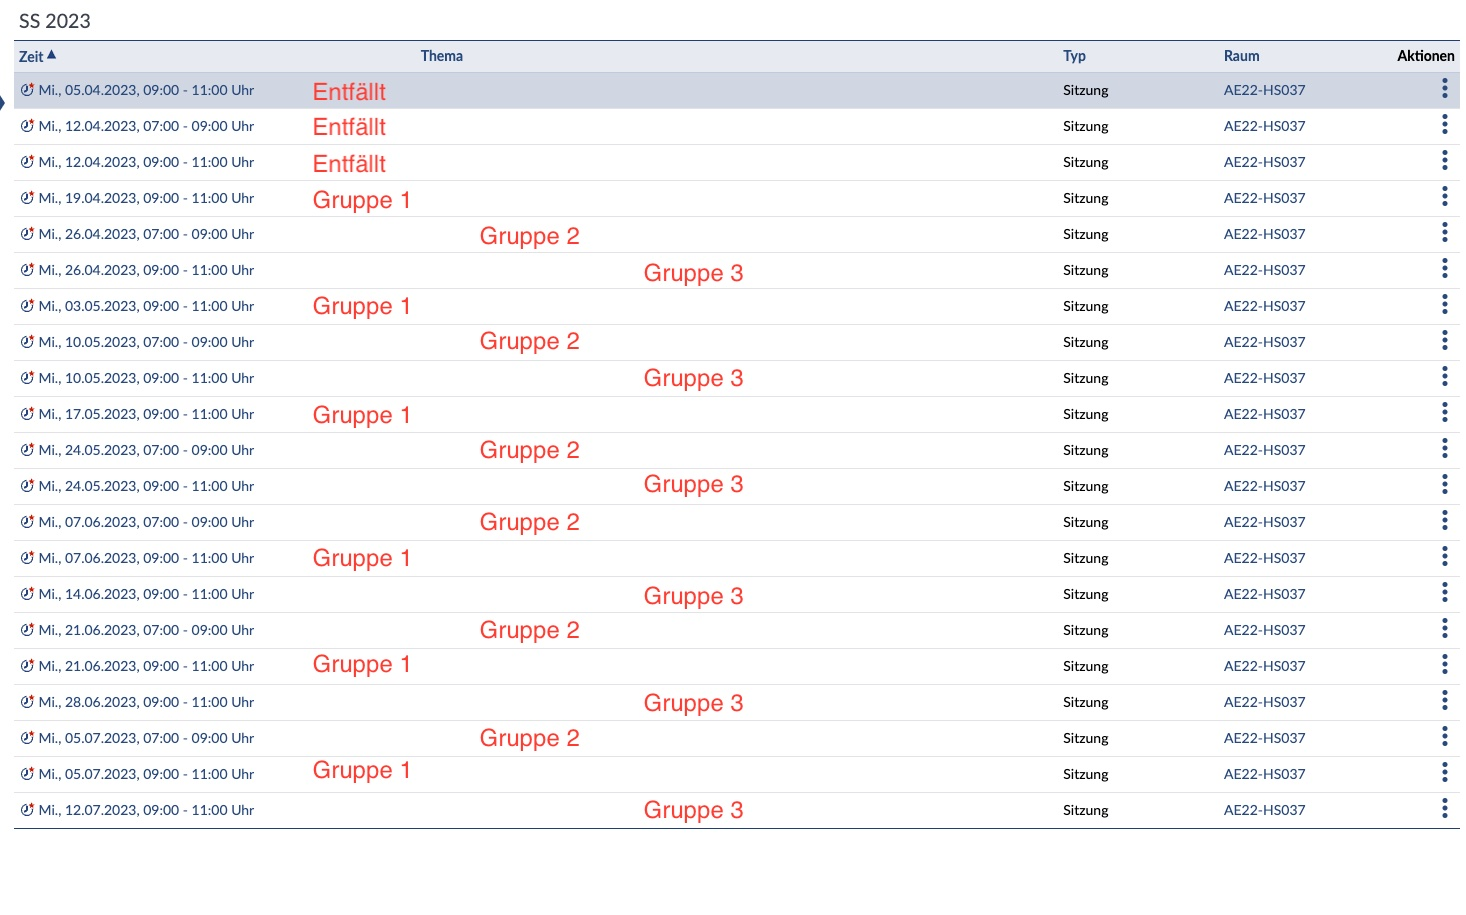
\includegraphics[scale=0.35,angle=90,origin=c]{zeitplan-studip-2023.jpg}
\end{center}
\caption{Abgleich mit der Planung auf StudIP.}
\end{figure}


\clearpage



\section{Didaktische Überlegungen}

Der Stil dieses Textes ist \textit{nicht} der Stil, den Sie für die eigene wissenschaftli\-che
Arbeit nutzen sollten. In einer wissenschaftlichen Arbeit ist der \textit{intersubjektive Schreibstil}
wichtig, 
während hier ein anderes, nämlich ein \textit{didaktisches und motivationelles} Ziel im Vordergrund steht.
Gleichwohl kann der Reader als Beispiel dienen, wie Texte gegliedert und satztechnisch
aufbereitet werden können.

Die Anforderungen an den
wissenschaftlichen Schreibstil werden wir im Laufe dieses Kurses besprechen.
Trotzdem wollen wir hier zur Abgrenzung einige Unterschiede nochmals besonders herausarbeiten:

\paragraph{Schreibstil:}
Mit meinem Stil hier versuche ich, Sie zu motivieren, Sie durch den Lesevorgang zu begleiten und die
Lektüre kurzweilig zu gestalten. Daher schreibe ich im persönlichen \textit{ich}-Stil,
nutze rhetorische Fragen, erzeuge gelegentlich einmal Widersprüche, bevor ich diese wieder auflöse usw.
Das soll den Text spannend machen und zum Nachdenken anregen.
In einer wissenschaftlichen Arbeit ist das nicht immer angebracht -- ausgenommen Sie verfolgen dort,
beispielsweise in der Einleitung oder in der Zusammenfassung ein ähnliches Ziel.

\paragraph{Layout:} Mit meinem Layout versuche ich, die Struktur und die Zusammenhänge
zwischen den einzelnen Lehrelementen herauszuarbeiten. Der Text soll dadurch leichter lesbar
werden. Sicher ist das auch ein sinnvolles Ziel für eine Belegarbeit. Andererseits sollte
eine Belegarbeit auch eine gewisse minimale Länger haben -- was einem Layout mit viel \enquote{Luft}
zuwiderläuft.

\paragraph{Fußnoten:}
Für die Informatik ungewöhnlich ist die intensive Nutzung von Fußnoten. Diese werden hier
gebraucht, um Kontexte zu Aussagen zu setzen, Dinge zu hinterfragen, nach einer 
überspitzten Formulierung wieder zurecht zu rücken, sowie um Zusatzinformationen zu geben.

In geisteswissenschaftlichen Arbeiten finden sich häufig sehr viele Fußnoten,
in den Ingenieur- und Naturwissenschaften stellen sie eher eher die Ausnahme dar.
Es handelt sich hier um eine Tradition der jeweiligen Disziplinen.
Zudem: In Wissenschaften, die überzeugt davon sind, die Dinge durch Definitionen formal präzise 
beschrieben zu können entsteht seltener der
Bedarf, zu kontextualisieren oder zurecht zu rücken.

\paragraph{Zitate:}
Dieser Reader arbeitet mit Hypertext-Links, die in PDF durch \LaTeX\ erzeugt werden. 
Wenn Sie ihn in einem Standard-kompatiblen
PDF-Reader betrachten, so können Sie direkt den farbigen Links folgen.

Diese Art der Einbindung von Zitaten orientiert sich an der digitalen Welt, ist auf
Webseiten und Blogs üblich und erlaubt einen raschen Zugriff auf die zitierte Stelle.
Aus wissenschaftlicher Sicht wäre das aus etlichen Gründen problematisch: Das Link-Ziel ist
einer auf Papier gedruckten Version des Readers nicht immer zu entnehmen\footnote{Der Reader behebt dieses 
Problem teilweise,
indem er -- meistens -- auch ein vollständiges Literaturzitat angibt. Diese Vorgehensweise ist
in einer wissenschaftlichen Arbeit jedenfalls erforderlich.}; 
ein Link ist manchmal sehr lang oder enthält viele Sonderzeichen und ist damit 
nicht gut für den menschlichen Gebrauch
oder den Abdruck in einem Dokument geeignet\footnote{In diesem Fall würde man in einer gedruckten
Arbeit den Link eher nicht einarbeiten, vorausgesetzt, das Literaturzitat ist durch die anderen Angaben
hinreichend präzise angegeben.}; Links bieten keine stabilen Zitate,
da sie sich ändern können (Versions-Problem), ganz verschwinden können (broken link)
oder nur kontextuell zugänglich sind (Cookies, pay walls).
Zudem zitiert der Reader mitten im Text und gelegentlich in Fußnoten, wie
es in Literatursammlungen üblich ist; in
wissenschaftlichen Arbeiten wird meistens mit einem Literaturverzeichnis gearbeitet.

Wie in wissenschaftlichen Arbeiten zitiert wird, finden Sie beispielsweise in der
\href{https://iuk.one/1012-1044.pdf}{Lerneinheit über wissenschaftliche Literatur https://iuk.one/1012-1044.pdf} genauer erklärt.
Eine Kombination der wissenschaftlichen Zitierweise mit Hypertext-Links 
ist für den Leser wissenschaftlicher Arbeiten sicher am bequemsten und daher anzustreben.

\paragraph{Flipped Classroom:} Die Entscheidung für die zumindest teilweise Nutzung des
\textit{flipped classroom} Modells folgt der lernpsychologischen Beobachtung, daß
man sich am besten jene Dinge merkt, die man sich selber erarbeitet hat. 
Ein Auswendiglernen von Begriffen oder Methoden bedeutet oftmals nur genau das: Begriffe und
Methoden werden nach der verbalen Präsentation des Dozenten verinnerlicht und die tiefere
Bedeutung der Begriffe und Modelle wird nicht erkannt. Dazu ist es erforderlich, daß man
die Konzepte sich selber sortiert, sie anwendet und erforderlichenfalls dabei
Rückmeldungen durch den Dozenten erhält. Zusätzlich regt diese Methode auch zu einem
laufenden Mitlernen während des Semesters an und ersetzt die sich sonst oft ergebende
Zweiphasen-Struktur eines Semester aus passivem Anhören gefolgt von Auswendiglernen.

\paragraph{\LaTeX\ Quellen:} Die meisten \LaTeX\ Quellen dieses Dokuments sind im
Github Repository \url{https://github.com/clecap/vorlesung-informatik-und-wissenschaft} zugänglich.
Sie haben damit auch ein Beispiel für ein längeres \LaTeX\ Dokument,
für die Nutzung diverser \LaTeX-Pakete und dafür,
wie bestimmte \LaTeX-Aufgaben gelöst werden können.

Lassen Sie sich aber nicht durch die Komplexität dieser Datei abschrecken! In diesem Dokument
bestanden nämlich eine ganze Reihe komplizierter Zusatzanforderungen. So mußten
beispielsweise externe PDF-Dateien eingebunden werden und \LaTeX-Programme 
innerhalb eines \LaTeX-Dokuments abgebildet werden.
Ebenso werden viele Verlinkungen und automatische Referenzen genutzt.


\paragraph{Fehler:} Wenn Sie in diesem Dokument Fehler finden oder Verbesserungsmöglichkeiten sehen,
tragen Sie diese bitte als Issue im Github Repository ein:

Hinweise auf Fehler im Dokument bitte im Repository \url{https://github.com/clecap/vorlesung-informatik-und-wissenschaft}
als \href{https://github.com/clecap/vorlesung-informatik-und-wissenschaft/issues}{\textit{issue}} einpflegen.

\clearpage

\hypertarget{Digitalvorlesung}{}
\section{Digitalvorlesungen}\label{Digitalvorlesung}\label{DV}

%% Macro zum Einbinden einer IDgitalvorlesung
% #1 Titel zur Ausgabe
% #2 URL Link nach Youtube, kompletter \url link
% #3 URL String für PDF Skriptum, nur string
% #4 Dauer in Minuten 

\def\video#1#2#3#4{\textbf{#1}\newline{\textbf{Video:}\tabto{2cm}\faYoutubePlay~#2 (Dauer #4)}%
\newline\textbf{Skriptum:}\href{#3}{\tabto{2cm}\faFilePdfO~\tt #3} }


\subsection{DV1: Wissenschaftliches Arbeiten mit Literatur}

\video{Wissenschaftliches Arbeiten mit Literatur}{\url{https://youtu.be/9GuG2AbmfNA}}{https://iuk.one/1012-1044.pdf}{2:52:00}

\subsection{DV2: Quantitatives wissenschaftliches Arbeiten}

\video{Quantitatives wissenschaftliches Arbeiten}{\url{https://youtu.be/RF_g_CHkQX8}}{https://iuk.one/1012-1050.pdf}{0:38:00}

\subsection{DV3: Stilistische Fragen beim Schreiben}

\video{Stilistische Fragen beim Schreiben \newline einer wissenschaftlichen Arbeit}{\url{https://youtu.be/s_RMbU36LC0}}{https://iuk.one/1012-1052.pdf}{0:28:00}

\subsection{DV4: Wissenschaft im Fallbeispiel}

\video{Wissenschaft im Fallbeispiel: \newline Was ist und wie arbeitet Wissenschaft?}{\url{https://youtu.be/tbodCUsUra4}}{https://iuk.one/1012-1046.pdf}{1:58:00}

\subsection{DV5: Anforderungen an eine wissenschaftliche Arbeit}

\video{Anforderungen an eine wissenschaftliche Arbeit}{\url{https://youtu.be/AecVy5rMG9M}}{https://iuk.one/1012-1049.pdf}{1:06:00}

\vspace*{\fill}

\textbf{Pro-Tipp:} Wir behandeln die einzelnen Themen in Vorlesung und Übung zwar linear, es gibt aber eine gewisse wechselseitige Abhängigkeit. Daher ist es sinnvoll,
die Inhalte nicht erst am Tag vor der jeweiligen Veranstaltung vorzubereiten, sondern etwas stärker vorausschauend. Das betrifft nicht nur die Digitalvorlesung, sondern auch den Reader.

\clearpage

\clearpage
\section{Präsenzvorlesungen}\label{Prsenzvorlesung}





\subsection{VL 1: Einführung. Wissenschaft, Lernen und \LaTeX}\glabel{VLIW1}

\textbf{Vorher ansehen:} Nichts. Ist ja die erste Veranstaltung überhaupt. \faSmileO\footnote{Knobelaufgabe: Wie setzen Sie
in \LaTeX\ ein solches Smiley?}

\bigskip

\textbf{Ablauf:}
\begin{enumerate}
\item \hyperref[ZieleUndInhalte]{Ziele und Inhalte}.
\item \hyperref[OrganisationUndAblauf]{Organisation und Ablauf}.
\item Kurzvortrag zu wissenschaftlicher Methodik.
\item Vortrag zu \href{https://iuk.one/1113-1001.pdf}{Lernstrategien (Link führt zum PDF Skriptum)}.
\item Vortrag \href{https://iuk.one/1112-1001.pdf}{Einführung zu \LaTeX\ (Link führt zum PDF Skriptum)}.
\end{enumerate}

\bigskip

\textbf{Nachbereitung:}
\begin{enumerate}
\item \useunit{Materialien zu Latex} (Hier: Sich einen Überblick über die bestehenden Materialien verschaffen und sich jene auswählen, mit denen man selber
im Semester arbeiten wird).
\item \useunit{Schnellesen} (Hier: Einige Tricks, um größere Mengen an Lesestoff zu bewältigen).
\item \useunit{Was ist Wissenschaft?} (Hier: Die ersten beiden Beiträge zu Cargo Cult Wissenschaft, die im Kurzvortrag zu wissenschaftlicher Methodik erwähnt wurden).
\end{enumerate}



\clearpage
\subsection{VL 2: Literatur 1}\glabel{VLIW2} 


\textbf{Vorher ansehen:}
\begin{enumerate}
\item \hyperlink{Digitalvorlesung}{Digitalvorlesung: Wissenschaftliches Arbeiten mit Literatur}
\item \useunit{Wissenschaftliche Literatur}
\end{enumerate}


\bigskip

\textbf{Aufgaben:}
\begin{enumerate}
\item \useaufgabe{ZitateVerbessern}
\end{enumerate}



\bigskip



\textbf{Kontrollfragen zur Präsenzvorlesung 1\footnote{Wir hatten in der Präsenzvorlesung 1 keine Vorbereitung, sondern nur eine
Nachbereitung. Diese Kontrollfragen beziehen sich auf diese Nachbereitung. Die weiter unten angeführten Kontrollfragen
beziehen sich auf die Vorbereitung dieser Präsenzvorlesung 2. Ebenso sind die Kontrollfragen bei den weiteren Präsenzvorlesungen zu verstehen.}:}
\begin{enumerate}
\item Was ist eigentlich eine \enquote{wissenschaftliche Methode}?
\item Woher wissen wir, ob eine wissenschaftliche Methode \enquote{richtig} ist?
\end{enumerate}
\bigskip


\textbf{Kontrollfragen:}
\begin{enumerate}
\item Warum ist Literaturarbeit überhaupt so wichtig?
\item Wie finden wir Quellen?
\item Ist die Angabe einer DoI im Literaturverzeichnis ausreichend? (ja/nein).
Argumentation?
\item Ist die Angabe der Auflage und/oder des Erscheinungsdatums bei einem Buch wichtig? (ja/nein). 
Argumentation?
\item Ist die automatisch Übernahme bibliographischer Metadaten aus dem Internet (z.B.: Google Scholar) ausreichend? (ja/nein).
Argumentation?
\item Wenn ich mit ChatGPT recherchiere, muß ich das dann zitieren? (ja/nein).
Argumentation?
\item Wie zitieren wir:  Blogs, Wikipedia, Internet-Quellen, Google, ChatGPT und ähnliche textgenerierende KI-Systeme?
\item Im Abschnitt \enquote{Stand der Technik} führe ich an, was in der Literatur zum Thema bekannt ist. Dazu lese ich Literatur, beschreibe das dort Erklärte und
füge ein Literaturzitat an. Reicht das aus? (ja/nein). Argumentation?
\end{enumerate}


\clearpage
\subsection{VL 3: Literatur 2}\glabel{VLIW3}


\textbf{Vorher ansehen:}
\begin{enumerate}
\item \hyperlink{Digitalvorlesung}{Digitalvorlesung: Wissenschaftliches Arbeiten mit Literatur}
\item \useunit{Wissenschaftliche Literatur}

\end{enumerate}


\bigskip

\textbf{Aufgaben:}
\begin{enumerate}
\item \useaufgabe{LiteraturBewerten}
\item \useaufgabe{Predator}
\end{enumerate}


\bigskip


\textbf{Kontrollfragen:}
\begin{enumerate}
\item Warum ist die Bewertung von Quellen wichtig?
\item Wie bewerten wir Quellen? Warum gehen wir dabei so vor?
\item Was bedeutet \textit{peer reviewed}? An welchen Merkmalen stellt man das fest?
\item Ist die Wikipedia nicht auch \textit{peer reviewed}? (ja/nein). Argumentation?
\item Was bedeutet wissenschaftlich qualitätsgesichert? An welchen Merkmalen stellt man das fest?
\item Was sind in der Informatik typische Beispiele guter Quellen?
\item Wir erarbeiten uns eine Checkliste zur Bewertung wissenschaftlicher Literatur.
\item Wir haben in der Belegarbeit eine Quelle verwendet, die wissenschaftlich nicht besonders wertvoll erscheint. Zitieren wir diese Quelle? (ja/nein).
Argumentation?
\item Wir verwenden in der Belegarbeit Informationen, die wir aus einer Grundlagenvorlesung entnehmen. Zitieren wir das Vorlesungsmanuskript? (ja/nein).
Argumentation?
\item Wir verwenden in der Belegarbeit Informationen, die wir aus der Wikipedia entnehmen. Zitieren wir den Artikel? (ja/nein)
Diskussion!





\end{enumerate}



\clearpage
\subsection{VL 4: Wissenschaft: Quantitatives Arbeiten und Schreiben}\glabel{VLIW4}


\textbf{Vorher ansehen:}
\begin{enumerate}
\item \hyperlink{Digitalvorlesung}{Digitalvorlesung: Stilistische Fragen beim Schreiben einer wissenschaftlichen Arbeit}.
\item \hyperlink{Digitalvorlesung}{Digitalvorlesung: Quantitatives wissenschaftliches Arbeiten}.
\item \useunit{Sprachlicher Ausdruck}
\item \useunit{Schreiben auf Englisch}
\end{enumerate}



\bigskip

\textbf{Aufgaben:}
\begin{enumerate}
\item \useaufgabe{EmpirischeDaten}
\item \useaufgabe{Zeitmessung}
\item \useaufgabe{sema}
\item \useaufgabe{Interpol}
\item \useaufgabe{Skinterpol}
\item \useaufgabe{Notensystem}

\end{enumerate}


\textbf{Kontrollfragen:}
\begin{enumerate}
\item Worin bestehen die typischen Probleme bei Interpolation und Extrapolation?
\item Bei welchen Skalen machen Interpolationen bzw. Extrapolationen Sinn?
\end{enumerate}



\clearpage
\subsection{VL 5: Wissenschaft: Methodik}\glabel{VLIW5}

\bigskip

\textbf{Vorher ansehen:}
\begin{enumerate}
\item \hyperlink{Digitalvorlesung}{Digitalvorlesung: Wissenschaft im Fallbeispiel}
\item \useunit{Methodische Fehler}

\end{enumerate}



\bigskip

\textbf{Aufgaben:}
\begin{enumerate}
\item \useaufgabe{Datenbereinigung}
\item \useaufgabe{Sonne}
\item \useaufgabe{GenauesFormulieren}
\item \useaufgabe{Experiment}
\item \useaufgabe{KognitiveVerzerrungen}
\end{enumerate}


\bigskip


\textbf{Kontrollfragen:}
\begin{enumerate}
\item Was ist eigentlich eine \enquote{wissenschaftliche Methode}?
\item Woher wissen wir, ob eine wissenschaftliche Methode \enquote{richtig} ist?
\item Was bedeutet Korrelation?
\item Was bedeutet Kausation?
\item Wie unterscheiden wir Korrelation von Kausation?
\end{enumerate}



\clearpage
\subsection{VL 6: Wissenschaft: Anforderungen}\glabel{VLIW6}

\textbf{Vorher ansehen:}
\begin{enumerate}
\item \hyperlink{Digitalvorlesung}{Digitalvorlesung: Anforderungen an eine wissenschaftliche Arbeit}
\item \useunit{Was ist Wissenschaft?}
\end{enumerate}


\bigskip

\textbf{Aufgaben:}
\begin{enumerate}
\item \useaufgabe{Anforderungen}

\item \useaufgabe{Papier}
\end{enumerate}



\bigskip


\textbf{Kontrollfragen:}
\begin{enumerate}


\item Welche Probleme entstehen bei der Verwendung textgenerativer Werkzeuge (Bsp: ChatGPT) in Bezug auf die Anforderungen an eine wissenschaftliche Arbeit?
\item Bewerten Sie nach den 10 Anforderungen an technische Arbeit die folgenden Artefakte:
\begin{enumerate}
\item Selbstfahrende Kraftfahrzeuge im SInne dieser beiden Beiträge: \url{https://www.tagesschau.de/wissen/technologie/selbstfahrende-autonome-autos-autobahn-101.html}
\url{https://de.wikipedia.org/wiki/Selbstfahrendes_Kraftfahrzeug}.
\item Die Google Suchmaschine
\item Das textgenerative Werkzeug ChatGPT.
\end{enumerate}
\item Wo liegen Grenzen der empirischen wissenschaftlichen Methode?

\end{enumerate}



\clearpage
\section{Übungen}\label{Ubung}



\subsection{Übung 1: \LaTeX und Wissenschaft}\glabel{UEIW1}

\textbf{Themen:}
\begin{enumerate}
\item Organisation und Ablauf der Veranstaltung
\item \textbf{\LaTeX:} Erste Einführung
\item \textbf{Wissenschaft:} Selbstreflexion über Wissenschaft: 
\begin{itemize}
\item[(a)] Was ist für mich Wissenschaft? 
\item[(b)] Was erwarte ich, was Wissenschaft leisten kann?
\end{itemize}
\end{enumerate}

\bigskip

\textbf{Vorführung:} \usedemo{ErsteSchritte}

\bigskip

\textbf{Aufgaben vorbereiten:}
\begin{enumerate}
\item \uselatexaufgabe{LatexTraining1}
\end{enumerate}

\bigskip

\textbf{Relevante Abschnitte im Reader:}
\begin{enumerate}
\item \useunit{Materialien zu Latex}, nach Bedarf der aktuellen Aufgaben
\item \useunit{Was ist Wissenschaft?}
\end{enumerate}




\clearpage


\subsection{Übung 2: Literatur, Organisieren und \LaTeX}\glabel{UEIW2}

\textbf{Themen:}
\begin{enumerate}
\item \textbf{Literatur:} Einführung in das Arbeiten mit Literatur.
\item \textbf{Organisieren:} Selbstorganisation und Zeitplanung.
\item \textbf{\LaTeX:} Dokumente.
\item \usedemo{Literatur}
\end{enumerate}

\bigskip

\textbf{Vorführung:} \usedemo{Literatur}

\bigskip

\textbf{Aufgaben vorbereiten:}
\begin{enumerate}
\item \uselatexaufgabe{LatexTraining2}
\item Nachdenken zum \hyperlink{Hausarbeit1}{1. Teil der Hausarbeit: Reflexion Studienziel}.
\end{enumerate}

\bigskip

\textbf{Relevante Digitalvorlesung:}
\begin{enumerate}
\item \hyperlink{Digitalvorlesung}{Digitalvorlesung: Wissenschaftliches Arbeiten mit Literatur}.
\end{enumerate}

\bigskip

\textbf{Relevante Abschnitte im Reader:}
\begin{enumerate}
\item \useunit{Materialien zu Latex}, nach Bedarf der aktuellen Aufgaben
\item \useunit{Selbstorganisation und Zeitplanung}
\end{enumerate}


\clearpage
\subsection{Übung 3: Literatur, Lesen und \LaTeX}\glabel{UEIW3}

\textbf{Themen:}
\begin{enumerate}
\item \textbf{Literatur:} Arbeiten mit wissenschaftlicher Literatur, Erfassen und Verarbeiten von Literaturdaten
\item \textbf{Lesen:} Techniken des erfassenden Lesens 
\item \textbf{\LaTeX:} Arbeiten mit \BibTeX, Einführung in \tikz\  und \textsc{pgf}
\end{enumerate}

\bigskip

\textbf{Vorführung:} \usedemo{Erfassen}

\bigskip

\textbf{Aufgaben vorbereiten:}
\begin{enumerate}
\item \uselatexaufgabe{LatexTraining3}
\item \useaufgabe{LiteraturSuche}
\item \useaufgabe{Suchen}
\end{enumerate}


\bigskip


\textbf{Relevante Digitalvorlesung:}
\begin{enumerate}
\item \hyperlink{Digitalvorlesung}{Digitalvorlesung: Wissenschaftliches Arbeiten mit Literatur}.
\end{enumerate}

\bigskip

\textbf{Relevante Abschnitte im Reader:}
\begin{enumerate}
\item \useunit{Materialien zu Latex}, nach Bedarf der aktuellen Aufgaben
\item \useunit{Lesen}
\end{enumerate}


\clearpage
\subsection{Übung 4: Schreiben und \LaTeX}\glabel{UEIW4}

\textbf{Themen:}
\begin{enumerate}
\item \textbf{Schreiben:} Schreibstil und Formulieren in wissenschaftlichen Arbeiten
\item \textbf{\LaTeX:} Abbildungen erstellen in \tikz\  und \textsc{pgf}
\end{enumerate}

\bigskip


\textbf{Aufgaben vorbereiten:}
\begin{enumerate}
\item \uselatexaufgabe{LatexTraining4}
\item \useaufgabe{FormVerbessern}
\end{enumerate}

\bigskip

\textbf{Relevante Digitalvorlesung:}
\begin{enumerate}
\item \hyperlink{Digitalvorlesung}{Digitalvorlesung: Stilistische Fragen beim Schreiben}.
\end{enumerate}

\bigskip

\textbf{Relevante Abschnitte im Reader:}
\begin{enumerate}
\item \useunit{Materialien zu Latex}, nach Bedarf der aktuellen Aufgaben
\item \useunit{Sprachlicher Ausdruck}
\item \useunit{Schreiben auf Englisch}
\end{enumerate}


\pagebreak
\subsection{Übung 5: Vortragen und \LaTeX}\glabel{UEIW5}

\textbf{Themen:}
\begin{enumerate}
\item \textbf{Vortragen:} Vorbereitung eines wissenschaftlichen Kurzvortrags
\item \textbf{\LaTeX:} Vortragsfolien in \LaTeX
\end{enumerate}

\bigskip


\textbf{Aufgaben vorbereiten:}
\begin{enumerate}
\item \uselatexaufgabe{LatexBeamer}
\item Nachdenken zum \hyperlink{Hausarbeit2}{2. Teil der Hausarbeit: Checkliste Seminarvortrag}
\end{enumerate}

\bigskip

\textbf{Relevante Abschnitte im Reader:}
\begin{enumerate}
\item \useunit{Materialien zu Latex}, nach Bedarf der aktuellen Aufgaben
\item \useunit{Vortragen}
\end{enumerate}



\clearpage
\subsection{Übung 6: Wissenschaft, Paper und \LaTeX}\glabel{UEIW6}

\textbf{Themen:}
\begin{enumerate}
\item \textbf{Wissenschaft:} Anforderungen an eine wissenschaftliche Arbeit
\item \textbf{Paper:} Anwendung des Gerlenten zum Schreiben einer kurzen wissenschaftlichen Arbeit
\item \textbf{\LaTeX:} Einbinden von Code, Erzeugen von Verzeichnissen
\end{enumerate}

\bigskip

\textbf{Aufgaben vorbereiten:}
\begin{enumerate}
\item \uselatexaufgabe{LatexTraining6}
\item Nachdenken zum \hyperlink{Hausarbeit3}{3. Teil der Hausarbeit: Kurzpapier}.
\end{enumerate}

\bigskip


\textbf{Relevante Digitalvorlesungen:}
\begin{enumerate}
\item \hyperlink{Digitalvorlesung}{Digitalvorlesung: Anforderungen an eine wissenschaftliche Arbeit}.
\item \hyperlink{Digitalvorlesung}{Digitalvorlesung: Quantitatives wissenschaftliches Arbeiten}.
\end{enumerate}

\bigskip

\textbf{Relevante Abschnitte im Reader:}
\begin{enumerate}
\item \useunit{Materialien zu Latex}, nach Bedarf der aktuellen Aufgaben
\end{enumerate}


\clearpage

\section{Hausarbeit}\label{Hausarbeit}

Die Lehrveranstaltung \enquote{Informatik und Wissenschaft} wird prüfungsmäßig durch eine
Hausarbeit abgeschlossen.  Diese Prüfungsleistung wird nicht
numerisch benotet sondern nur als \enquote{bestanden} oder \enquote{nicht bestanden} gewertet.
Es gibt keine mündliche Prüfung und keine Klausur.

Die Hausarbeit besteht aus drei kurzen Arbeitsproben, in denen sie die Kernkompetenzen dieser
Veranstaltung einüben und nachweisen.

{\textbf{Wichtig:} Die Abgabe erfolgt per Email in Form einer einzigen PDF-Datei, welche die drei unten beschriebenen
Arbeitsproben zusammenfaßt. Die Datei muß spätestens bis zum 15. Juli beim Leiter Ihrer Übungsgruppe
eingetroffen sein.

\textbf{Hinweise:}
Sie müssen alle drei Teildokumente der Hausarbeit \textit{persönlich und alleine} erstellen;
sie dürfen nicht in Zusammenarbeit oder gemeinsam mit anderen Studenten erarbeitet werden.

Die Nutzung von Suchmaschinen bei der Recherche ist sinnvoll und zulässig. Auf die Regelungen für Zitate,
Wortzitate und Plagiate wird ausdrücklich hingewiesen, da diese Lehrinhalte dieses Moduls sind.

Der Einsatz von ChatGPT und ähnlichen Werkzeugen kann \textit{teilweise} sinnvoll sein, führt aber 
erfahrungsgemäß auch zu einer Verengung von
Perspektiven auf Mehrheitsmeinungen, soweit diese in Texten im World Wide Web verfügbar sind;
ebenso können beim Einsatz dieser Systeme massive Fehler auftreten.
In jedem Fall bleiben Sie als Autor endverantwortlich für die dargelegten Aussagen und Argumente.

Die Nicht-Beachtung dieser Hinweise kann zu einer negativen Bewertung der Hausarbeit führen;
Plagiate können einen Eintrag als Betrugsversuch in die Akte im Studienbüro nach sich ziehen.


\setcounter{aufgabencounter}{0}

\clearpage

\hypertarget{Hausarbeit1}{}
\subsection{Teil 1: \LaTeX\ Kurzdokument \& Reflexion Studienziel}\label{H1}

\textbf{Aufgabe:} Erstellen Sie ein kurzes Dokument (3-4 Seiten), 
das Ihre persönlichen Studienziele erläutert und erklärt, wie Sie diese erreichen wollen.

\textbf{Formatvorgabe:} \LaTeX, DIN A4, 11 Punkt Font, eigene Formatentscheidung.

\textbf{Ziele} dieser Aufgabe sind:
\begin{enumerate}
\item \textit{Eigenständige Gestaltung} eines vollständigen Kurzdokuments in \LaTeX.

Die Aufgabe bietet viele Möglichkeiten zur Einübung unterschiedlicher Formatierungstechniken von \LaTeX\ 
(Titelgestaltung, Gliederung, Hervorhebung, Tabelle, Liste usw.) Diese sollten genutzt werden und dem Inhalt entsprechend
angepaßt sein.

\item \textit{Reflexion} über die Ziele Ihres Studiums und Umsetzung in eine Planung. 

Mögliche inhaltliche 
Schwerpunkte können dabei sein: Warum studiere ich das, was ich studiere? 
Was plane ich nach dem Bachelor-Abschluß?
Welche inhaltlichen, zeitlichen und organisatorischen Schwerpunkte folgen daraus? Welche besonderen Schwierigkeiten und Herausforderungen
erkenne ich bereits heute? Wie will ich diese meistern?
Woran erkenne ich, ob ich im Plan bin? Wie würde ich auf erkannte Planabweichungen reagieren? 

Da es hier um Ihre eigene Reflexion geht, ist es nicht sinnvoll, sich Anregungen aus Internet-Blogs zu holen -- 
unabhängig, ob Sie diese dann zitieren oder nicht. Im letzteren Fall wäre es natürlich auch noch ein Plagiat.
\end{enumerate}

\clearpage

\hypertarget{Hausarbeit2}{}
\subsection{Teil 2: Checkliste Seminarvortrag}\label{H2}

\textbf{Aufgabe:} Erstellen Sie eine \textit{einseitige} Checkliste für Seminarvorträge für den Eigengebrauch.

\textbf{Formatvorgabe:} \LaTeX, DIN A4, 11 Punkt Font, eigene Formatentscheidung.

\textbf{Hinweise:}

\begin{enumerate}
\item Ein Seminarvortrag wird nicht deshalb gut, weil Sie Checkliste 17 beachtet haben und nicht Checkliste 23a,
sondern deshalb, weil Sie sich rechtzeitig Gedanken darüber gemacht haben, was bei einem Vortrag wirklich wichtig ist.
Dazu noch vor dem ersten eigenen Seminarvortrag anzuregen ist der Sinn dieser Aufgabe.

\item Es gibt nicht die eine, richtige Art und Weise eines Vortrags, aber es gibt eine ganze Reihe von Fehlern, die
man vermeiden möchte. Dabei kann eine Checkliste helfen.

\item Sehen Sie sich die Quellen im Reader auf Seite~\pageref{vortragen}ff. zu diesem Thema an. 
Suchen Sie weitere Hinweise im
Internet. Quellennachweise direkt in der Checkliste sind nicht erforderlich, da die Checkliste für den Eigengebrauch erstellt werden soll.
Wenn Sie allerdings nur Quellen zusammenkopieren, sich nicht über eine eigene Auswahl oder Gewichtung Gedanken
machen und auch keine eigenen Vorschläge einbringen, dann haben Sie die Aufgabe nicht richtig gelöst. 

\item Wenn in der Checkliste fremde Ideen verwendet werden, ist eine Liste benutzter Quellen auf einer separaten Seite anzufügen.
\end{enumerate}

\textbf{Ziele} dieser Aufgabe sind:
\begin{enumerate}
\item Sie beschäftigen sich mit verschiedenen Perspektiven, wie ein Seminarvortrag gestaltet werden soll.
\item Sie machen sich eigene Gedanken zu den Qualitätskriterien eines Seminarvortrags und treffen eine persönliche
Auswahlentscheidung.
\item Sie strukturieren das Ergebnis eigenständig -- und wie wir aus der Lerntheorie wissen, ist das die effizienteste
Form des Lernens.
\end{enumerate}

\clearpage

\hypertarget{Hausarbeit3}{}
\subsection{Teil 3: Kurzpapier}\label{H3}

\textbf{Aufgabe:} Erstellen Sie ein kurzes Dokument von 4-6 Seiten Textinhalt zu einem vorgegebenen Thema der Informatik.

\textbf{Formatvorgabe:} \LaTeX, DIN A4, 11 Punkt Font, doppelspaltiger IEEE-Stil.

Der doppelspaltige
IEEE-Konferenz-Stil ist ein in der Informatik sehr häufig benutzter Satz-Stil.
Weitere Informationen zu diesem Stil finden Sie 
auf der \href{https://www.ieee.org/conferences/publishing/templates.html}{Home\-page des Stils bei der IEEE}
\url{https://www.ieee.org/conferences/publishing/templates.html}.
Es gibt ein Musterdokument, das selber in diesem Stil geschrieben ist und zugleich als Howto
für diesen Stil dient.
\href{https://ftp.agdsn.de/pub/mirrors/latex/dante/macros/latex/contrib/IEEEtran/IEEEtran_HOWTO.pdf}{Howto
https://ftp.agdsn.de/pub/mirrors/latex/dante/macros/latex/contrib/IEEEtran/ IEEEtran\_HOW TO.pdf
}. Rund 95\% dieses Howto werden Sie nicht benötigen. Es dient uns hier aber als Muster für diesen Stil
und als Beispiel dafür, wie solche Formatvorgaben typischerweise aufgebaut sind.
Wenn Sie Overleaf als \LaTeX-Umgebung nutzen, so finden Sie weitere Informationen auf
\url{https://www.overleaf.com/gallery/tagged/ieee-official}.

\textbf{Anforderungen:} Das Dokument soll enthalten:
\begin{enumerate} \item mindestens eine Tabelle, 
\item mindestens eine Abbildung oder Grafik,
\item mindestens eine Fußnote, 
\item mindestens ein eingebundenes Beispielprogramm,
\item eine Titelseite, 
\item ein Inhaltsverzeichnis, 
\item ein Abbildungsverzeichnis, 
\item ein Tabellenverzeichnis und 
\item ein Literaturverzeichnis. 
\end{enumerate}

Titelseite, Verzeichnisse, Bilder und Tabellen werden \textit{nicht} auf die Seitenzahl des
Textinhalts angerechnet, da diese von \LaTeX\ automatisch erzeugt werden.

\textbf{Themenvorgabe:} Die Datenstruktur des Binärbaums und ihre Anwendung.

\textbf{Ziele} dieser Aufgabe sind:

\begin{enumerate}
\item Sie üben die wichtigen Grundfunktionen von \LaTeX\ in einem Dokument.
\item Sie erstellen ein Kurzdokument zu einem bekannten und einfachen Thema der
Informatik.
\item Sie vertiefen Ihr Wissen über eine der wichtigsten Datenstrukturen.
\item Sie wenden die in Vorlesung und Übung erarbeiteten Techniken zur Erstellung einer fachwissenschaftlichen Kurzarbeit an.
\item Sie üben die Nutzung eines vorgegebenen Dokumenten-Templates.
\end{enumerate}


\textbf{Zur Motivation:}
Es ist uns bewußt, daß es zu diesem Thema tausende verschiedener Dokumente im World Wide Web und im akademischen
Schrifttum gibt. Ziel dieser Aufgabe ist \textit{nicht}, diesen Dokumenten noch weitere hundert hinzuzufügen.
Wenn Sie aber später einen Projektbericht, eine Bachelor- oder Masterarbeit schreiben, dann ist es notwendig, daß
Sie sich mit den formalen und schreibtechnischen 
Fragen, die bei der Erstellung eines solchen Dokuments auftreten, schon einmal beschäftigt haben,
und die dafür erforderlichen Grundtechniken eingeübt haben.


\clearpage


\section{\LaTeX-Training}\label{latex}


Dieser Abschnitt enthält Aufgaben, anhand derer wir uns in den Übungen in \LaTeX\ einarbeiten werden.
In jeder Übung werden wir eine \LaTeX-Trainingseinheit anhand einer praktischen
Anforderung bearbeiten, die im Informatik-Studium auftritt.


\latexaufgabe{\LaTeX-Training 1: Installation und Hello World}{LatexTraining1}

\textbf{Einführende Aufgaben:}
\begin{enumerate}
\item Informieren Sie sich über \LaTeX-Installationen, die für Ihr Rechnersystem verfügbar sind.
\item Wählen Sie eine geeignete \LaTeX-Installation aus.
\item Installieren Sie diese auf Ihrem Rechner.
\item Erstellen Sie ein einfaches \enquote{Hello World} Dokument und wandeln Sie dieses in eine PDF-Datei um.
\end{enumerate}


\latexaufgabe{\LaTeX-Training 2: Übungsdokument}{LatexTraining2}

Erstellen Sie Übungsdokumente, in denen Sie die folgenden Funktionen von \LaTeX\ an 
jeweils zwei Beispielen ausprobieren:

\textbf{Teilaufgaben:}
\begin{enumerate}
\item Textauszeichnungen wie beispielsweise \textbf{fett}, \textit{kursiv}, \underline{unterstrichen} oder {\color{red}farbig}. 

\textbf{Zusatzfrage:}\footnote{\LaTeX\ kann sehr viel. Als Programmiersprache ist es sogar \textsc{Turing}-vollständig und kann beispielsweise die
ersten hundert Dezimalstellen von $\pi$ berechnen. Das Lernziel bei den Zusatzfragen ist, zu üben, wie und wo Sie im Internet
bei \LaTeX-Fragen Hilfe finden können. Wir müssen Werkzeuge nicht perfekt beherrschen -- wir müssen aber wissen,
wie wir neue Anforderungen mit den Werkzeugen erfüllen, wenn sie bei unserer Arbeit auftauchen.} Wie können Sie in \LaTeX\ selber neue Farben definieren?
\item Tabellen. Probieren Sie aus, wie Sie die Abstände zwischen den Zeilen und
  Spalten anpassen können, wie einzelne Zellen mal linksbündig und mal rechtsbündig gesetzt werden können, wie einfache und doppelte
  Linien gezeichnet werden und wie Zellen eingefärbt werden können.
\item Abschnitte von Dokumenten (etwa: \texttt{\textbackslash section} und \texttt{\textbackslash subsection}) und 
 ein automatisch erzeugtes Inhaltsverzeichnis. 

 \textbf{Zusatzfrage:} Wie können Sie die Formatierungen \texttt{\textbackslash section} oder \texttt{\textbackslash subsection}
 nutzen, ohne daß diese im Inhaltsverzeichnis aufscheinen?
\item Automatisch erzeugte Titelseite mit \texttt{\textbackslash maketitle}.
\item Einbinden einer Abbildung im PNG, SVG und PDF Format. Wie können Sie die Abbildung skalieren und im Dokument mittig 
positionieren?

\textbf{Zusatzfrage:} Wie können Sie mehrere Abbildungen nebeneinander darstellen?
\item Nutzung der Silbentrennung mit eingebundener Trenntabelle der benutzten Sprache.
\end{enumerate}


\latexaufgabe{\LaTeX-Training 3: Amplituden-Modulation}{LatexTraining3}

In einer Bachelorarbeit soll die Amplituden-Modulation dargestellt werden.
Dazu besteht bereits die folgende Abbildung:

\begin{figure}[h]
\begin{center}
\begin{tikzpicture}
  \begin{axis}[]
    \addplot[ domain = 0:30 ]  {exp(-x/10)*( cos(deg(x)) ) }; % Hochfrequenz
    \addplot[ domain = 0:30 ]  {exp(-x/10)};                  % Obere Hüllkurve
    \addplot[ domain = 0:30 ]  {-exp(-x/10)};                 % Untere Hüllkurve
\end{axis}
\end{tikzpicture}
\end{center}
\end{figure}

\begin{minted}{latex}
\begin{tikzpicture}
  \begin{axis}[]
    \addplot[ domain = 0:30 ]  { exp(-x/10)*( cos(deg(x)) ) }; % Hochfrequenz
    \addplot[ domain = 0:30 ]  { exp(-x/10)  };                % Obere Hüllkurve
    \addplot[ domain = 0:30 ]  { -exp(-x/10) };                % Untere Hüllkurve
\end{axis}
\end{tikzpicture}
\end{minted}

\textbf{Aufgabe:} Verbessern Sie die Abbildung. Konkret:
\begin{enumerate}
\item Die Hochfrequenz ist doch ziemlich eckig.
\item Die Frequenzkurve sollte die Hüllkurve berühren!\newline
  Warum sollte sie das? Warum tut sie das hier nicht? Wie reparieren Sie das?
\item Die Hüllkurven sollten von der Hochfrequenz besser abgegrenzt sein. Wir können sie dazu in einer anderen Farbe oder
strichliert zeichnen.
\item Eine Null-Linie würde das Bild noch etwas verbessern.
\item Die Abbildung benötigt noch eine Legende und eine Figure-Caption zur Erläuterung.
\end{enumerate}

Erstellen Sie ein Dokument, in dem diese Probleme behoben sind.

\textbf{Hinweis:} Diese Aufgabe nutzt verschiedene Zusatzpakete, die Sie beispielsweise mit dieser Anweisung
einbinden können:
\texttt{\textbackslash usepackage\{tikz,pgfplots\}}. Auch die weiteren Aufgaben benötigen ggf.\ Zusatzpakete.


\latexaufgabe{\LaTeX-Training 4: \tikz\  und \textsc{pgf}}{LatexTraining4}

Die folgende Tabelle und der nebenstehende Graph beschreiben einen
endlichen Automaten, der genau alle Wörter über dem Alphabet $\{ 0,1\}$ akzeptiert,
die ein oder mehr Zeichen \enquote{0} enthalten.

\begin{tabular}[]{lll}
\textbf{Zustand} & \textbf{Input} & \textbf{Folgezustand} \\
 $A$ & $0$ & $B$ \\
 $A$ & $1$ & $A$ \\
 $B$ & $0$ & $B$ \\
 $B$ & $1$ & $B$
\end{tabular}
\begin{tikzpicture}[node distance=2cm]
\node[state, initial]                  (s1) {$A$};
\node[state, accepting, right of=s1]   (s2)  {$B$};
\draw (s1)  edge[loop above] node{1}   (s1);
\draw[->] (s1)  edge[bend left, above] node{0}   (s2);
\draw (s2) edge[loop above] node{$0,1$} (s2);
\end{tikzpicture}

\textbf{Aufgaben:}
\begin{enumerate}
\item Erstellen Sie diese Tabelle und den Graphen.
\item Machen Sie das Layout der Tabelle schöner: Die Tabelleneinträge sehen horizontal zentriert besser aus, 
das Wort \enquote{Folgezustand} ist zu breit und
könnte als \enquote{Folge-zustand} umgebrochen werden -- dann allerdings wird der Tabellenkopf zweizeilig und man
würde sich nun eine vertikale Zentrierung aller Kopfzellen wünschen. Vielleicht möchte man Trennlinien oder einen Rahmen einzeichnen.
\item Verbessern Sie das Layout insgesamt:
Der Graph sollte vertikal mittig zur Tabelle gesetzt sein, in 
einem sinnvollen Abstand. Alles sollte auf der Seite horizontal zentriert stehen. Das Wort \enquote{start} sollte mit einem großen 
\enquote{S} beginnen. Wir benötigen eine \texttt{\textbackslash caption} und einen Label, um die Tabelle referenzieren zu können.
Wenn die Start-Zustände und die End-Zustände im Hintergrund farbig unterlegt sind, dann läßt sich der
Graph leichter lesen. 
\item Erstellen Sie nun die Beschreibungs-Tabelle und den Graphen für einen endlichen Automaten,
der genau alle Wörter über dem Alphabet $\{0, 1\}$ akzeptiert, die eine durch drei teilbare Anzahl von Einsern enthalten.
\end{enumerate}



\latexaufgabe{\LaTeX-Training 5: Beamer}{LatexBeamer}

Erstellen Sie eine eine 3-Folien-Kurzpräsentation mit \LaTeX-Beamer über das Thema \enquote{Model-View-Controller}.
Wir benötigen:

\begin{enumerate}
\item Eine Titelfolie mit Namen, Vortragstitel, Datum usw.
\item Eine Folie mit Text.
\item Eine Folie mit einer selbst gezeichneten Abbildung.
\end{enumerate}

\textbf{Anleitung:}
\begin{enumerate}
\item Für Abbildungen lassen Sie sich vom Internet inspirieren:
\url{https://duckduckgo.com/?q=model+view+controller&iax=images&ia=images}

\item Zur Umsetzung der Abbildung gibt es viele Möglichkeiten:
\href{https://texample.net/tikz/examples/smart-flowchart/}{Mit Smartdiagram}
oder mit
\href{https://texample.net/tikz/examples/borrowers-and-lenders/}{\tikz}. Starten Sie mit einem
Beispiel und arbeiten Sie sich von dort aus weiter.

\item Für die Erklärung des Design-Musters Model-View-Controller greifen Sie auf entsprechende Vorlesungen zu Programmierung 
zurück oder nutzen Beschreibungen im Internet oder von Wikipedia.

\item Zu \LaTeX-Beamer finden Sie Informationen im Reader auf Seite \pageref{latexbeamermaterial}.
\item Ihrer Fantasie ist nun keine Grenze mehr gesetzt: Wollen Sie einen eleganten Footer? Ein schöneres Template? Nutzen Sie
die Aufgabe, um \LaTeX-Beamer besser kennenzulernen.
\end{enumerate}


\latexaufgabe{\LaTeX-Training 6: Code und Index}{LatexTraining6}

\begin{enumerate}
\item Installieren Sie auf Ihrem System das \LaTeX-Paket \texttt{minted} und die dazu gegebenenfalls noch erforderlichen 
Zusatzprogramme\footnote{Das ist nicht auf jedem System ganz einfach. Nehmen Sie die Herausforderung an: Mit Geduld und StackExchange 
finden Sie eine Lösung und lernen dabei Ihr Betriebssystem, Pfade und \textit{Shebangs} besser kennen. Alternativ
können Sie das \texttt{minted} auf \href{www.overleaf.com}{Overleaf} nutzen oder das alternative Paket \texttt{listings} verwenden.}

\item Erstellen Sie ein kurzes Textdokument, in das Sie mittels \texttt{minted} oder \texttt{listings} ein kurzes Javascript Programm
und den Quelltext eines kurzen \LaTeX-Dokuments mittels Syntax Highlighting (\texttt{minted}) oder Quelltext-Formatierung (\texttt{listings}) einbinden.
Tipp: Optisch sieht das schön aus, wenn man das Ergebnis noch horizontal zentriert, in eine float Umgebung (\texttt{table} oder \texttt{figure})
verpackt und mit einer \texttt{\textbackslash caption} zur Erklärung versieht.
\item Fügen Sie in das Dokument noch einige Einträge für ein Schlagwortverzeichnis (Index) ein
und generieren Sie automatisch diesen Index.
\end{enumerate}

\textbf{Bonusfrage:} Wenn Sie den Code in eine \texttt{table} oder \texttt{figure} verpacken, dann scheint er auch
in der entsprechenden Tabelle auf. Geben Sie diese ebenso aus!

\textbf{Superbonusfrage:} Code als Teil einer \texttt{\textbackslash listoftables} vorzufinden ist nicht optimal.
Wäre es nicht schön, wenn wir ein neues \texttt{float} definieren könnten, etwa so:

\begin{figure}[h]
\centering
\begin{minipage}[b]{0.5\textwidth}
\begin{minted}{latex}
\begin{program}
... hier steht die minted Umgebung 
    mit dem Programmcode ...
\end{program}
\end{minted}
\end{minipage}
\caption{Beispiel für eine neue \LaTeX-Umgebung.}
\end{figure}

In diese Umgebung schreiben wir dann auch eine Beschreibung mit \texttt{\textbackslash caption} und
erzeugen uns am Ende der Arbeit eine \texttt{\textbackslash listofprograms}.
\LaTeX\ kann alles -- also geht auch das; wenn Sie es umgesetzt haben, dann sind Sie ein wahrer {\TeX}nician geworden.


\pagebreak




\section{Aufgaben} \hypertarget{Aufgaben}{}\label{auf}

Dieser Abschnitt enthält Aufgaben, die wir im Laufe der Veranstaltung
bearbeiten werden. 
Die \hyperref[Prsenzvorlesung]{Arbeitspläne der Präsenzvorlesung} und der \hyperref[Ubung]{Übung}
verweisen dabei auf die einzelnen Aufgaben.


\aufgabe{Zitate verbessern}{ZitateVerbessern}

In einer Arbeit finden Sie die folgenden Literaturangaben:

\begin{quote}
[44] Seoung Kim Measuring Ethereum Network Peers 2020.

[Dr.W] Dr. Wood, Ethereum. https://sands.kaust.edu.sa/classes/CS394B/S18/papers/ethereum.pdf

[ASpier2021] Alexander Spier: Ethereum schürfen leicht gemacht. Heise, 9. 3. 2021. 

[Wikipedia.En] Wikipedia: Ethereum. \url{https://en.wikipedia.org/wiki/E thereum},
PageId 41754003, Revision 1073898461 vom 25. 02. 2022, abgerufen 
am 25. 02. 2022.
\end{quote}



\textbf{Aufgabe:}
\begin{enumerate}
\item \textit{Welche} Probleme bestehen bei diesen Literaturangaben? Begründen Sie jeweils im Einzelnen, \textit{warum} das Probleme sind.
\item \textit{Beheben} Sie diese Probleme indem Sie eine korrekte Literaturangabe anfertigen. Erstellen Sie dazu eine
\BibTeX Datei, eine \LaTeX-Datei und schließlich eine PDF Datei. Wenn zur zitierten Arbeit ein Web-Link existiert,
dann soll die PDF Datei im Literaturverzeichnis auch auf die Arbeit mit einem klickbaren Link verweisen.
\item Wie bewerten Sie diese Zitate hinsichtlich ihrer Qualität? 
\item Wie oft wurden diese Arbeiten von anderen Arbeiten zitiert? \textit{Wie} gehen Sie bei der Beantwortung
dieser Frage vor? \textit{Warum} ist diese Vorgehensweise sinnvoll und vertrauenswürdig? 
\item Sind diese Arbeiten für ein wissenschaftliches Zitat geeignet? An welchen \textit{Kriterien} machen Sie
Ihre Entscheidung fest?
\item Sind diese Arbeiten wissenschaftlich qualitätsgesichert (peer review)?  An welchen \textit{Kriterien} machen Sie
Ihre Entscheidung fest?
\end{enumerate}






\aufgabe{Bewerten von Literaturstellen}{LiteraturBewerten}

\textbf{Aufgaben:}
\begin{enumerate}
\item Welche der im folgenden angegebenen 4 Literaturstellen sind von einer wissenschaftlich 
guten Qualität? 
\item Welche Kriterien verwenden wir dafür?
\item Warum sind diese Kriterien gut bzw.\ wann sind sie schlecht?
\end{enumerate}

\textbf{Hinweis:} Die Fragen nach den Kriterien, nach der Eignung der Kriterien und nach den Grenzen
ihrer Anwendbarkeit sind die drei unvermeidlichen Fragen, die wir uns als Wissenschaftler
\underline{\textbf{immer}} stellen müssen, auch wenn sie oft nicht explizit in der Aufgabenstellung stehen! 


\textbf{Die Literaturzitate:}
\begin{quote}
(1) M. Nguyen, H. Nguyen, K. Teague: Wavelet-based Energy Efficient Data 
Collection Algorithm in Wireless Sensor Networks. 
ICSES Transactions on Computer Networks and Communications, 
Vol 4 (2), 2018, pp 3-10,ISSN 2588-5847,
DOI: \href{https://doi.org/10.31424/icses.itcnc}{10.31424/icses.itcnc}

(2) J. Zhang, J. Guo, W. Su: TIC: A Methodology for the Construction of E-Commerce.
International Conference on Quality, Reliability, Risk, Maintenance, and
Safety Engineering (QR2MSE), 2013. DOI: \href{https://doi.org/10.1109/QR2MSE.2013.6626010}{10.1109/QR2MSE.2013.6626010}

(3) J. Stribling, D. Aguayo, M. Krohn: Rooter: A Methodology for the
Typical Unification of Access Points and Redundancy.
9th World Multi-Conference on Systemics, Cybernetics and Informatikcs (WMSCI),


(4) R. Mosallahnezhad: Cooperative, Compact Algorithms for Randomized Algorithms.
Applied Mathematics and Computation, Elsevier, 
ISSN 0096-3003, DOI: \href{https://doi.org/10.1016/j.amc.2007.03.011}{10.1016/j.amc.2007.03.011}
\end{quote}








\aufgabe{Predatory Publishers}{Predator}

Ist es sinnvoll, auf die nachfolgende Email zu reagieren? Warum? Warum nicht?

\textbf{Aufgabe:}
\begin{enumerate}
\item Welche Kriterien können wir benutzen, um einen \textit{publisher} zu bewerten?
\item Was ergibt sich bei einer Anwendung dieser Kriterien auf den unten angeführten Verlag?
\end{enumerate}

\textbf{Hinweis:} Es ist schon öfters vorgekommen, daß Studenten nach Abgabe und Veröffentlichung Ihrer Masterarbeit eine ähnliche
Mail erhalten haben.
Die in dieser Aufgabe eingeübten Fähigkeiten und Einschätzungen sind ebenso für die Beurteilung von
Literaturstellen sinnvoll, die Sie in einer Belegarbeit nutzen wollen.

\begin{quote}\em
Dear Dr. Cap,

Due to your involvement in the field and the research you published in your paper, 
"The limits of blockchain [Grenzen der Blockchain]," IntechOpen invites you to contribute a chapter to "Blockchain," an Open Access book edited by Dr. Vardan Mkrttchian.

Work with an internationally recognized peer group and gain increased visibility for your published work.
Please visit the book project page to start the submission process.

We look forward to hearing from you.

Kind Regards,

Romina Rovan
Author Service Manager

IntechOpen
Rijeka: Janeza Trdine 9, 51000 Rijeka, Croatia
London: 5 Princes Gate Court, London, SW7 2QJ, UK
+44 20 8089 5702

INTECHOPEN LIMITED, Registered in England and Wales No. 11086078

We are IntechOpen, the world's leading publisher of Open Access books
Built by scientists, for scientists
\end{quote}







\aufgabe{Suchen von Literatur}{LiteraturSuche}

\textbf{Aufgaben:}
\begin{enumerate}
\item Welche Arbeiten hat Clemens Cap zu Bitcoin veröffentlicht?
\item Suchen Sie alle Arbeiten heraus.
 Wie häufig wurden diese Arbeiten zitiert?
\item Erfassen Sie diese Arbeiten in einer Datei im \BibTeX Format.
\item Erstellen Sie ein Literaturverzeichnis, das alle diese Arbeiten anführt.
\end{enumerate}









\aufgabe{Suchen und Verarbeiten von Literaturstellen}{Suchen}

Sie benötigen von den folgenden vier Texten jeweils die veröffentlichte Originalversion als PDF-Dokument,
die vollständigen bibliographischen Daten und den DoI Link.
Sie haben dazu die folgenden Informationen:

\begin{enumerate}
\item Kapitel 2 \enquote{Sortieren und Suchen} aus dem Buch \enquote{Algorithmen und Datenstrukturen} von Helmut Knebl in der
neuesten an der UB Rostock verfügbaren Auflage.
\item Anika Mansura et. al: \enquote{An energy balanced and nodes aware routing protocol for energy harvesting wireless sensor networks}
\item Den Text \enquote{A Security Enhanced Verification Framework Based on Device Fingerprint} von Fu, Huang und Zhang.
\item Die Promotionsarbeit von Christian Bünnig an der Universität Rostock über Privacy Management.
\end{enumerate}

\textbf{Aufgaben:}
\begin{enumerate}
\item Besorgen Sie sich die PDF-Dateien dieser Literaturstellen.
\item Erstellen Sie eine Datei im \BibTeX-Format, welche die vollständigen bibliographischen Daten erfaßt (auch DOIs, wo solche existieren).
\item Erstellen Sie ein \LaTeX-Dokument, das diese vier Arbeiten zitiert und das ein Literaturverzeichnis enthält.
\item Konvertieren Sie das Dokument nach PDF und kontrollieren Sie es auf Satzfehler.
\end{enumerate}




\aufgabe{Darstellung empirisch gewonnener Daten}{EmpirischeDaten}

\textsc{Alice} und \textsc{Bob} 
bereiten einen Seminarvortrag über das Zeitverhalten von Sortierverfahren vor. Sie verwenden dazu das folgende Programm
in HTML / Javascript und lassen es im Browser laufen.

\begin{minted}{html}
<html><body><script>
function swap (arr, first, second) {
  arr [first]  = arr [second];
  arr [second] = arr [first];
}

function bubbleSort (arr) {
  var len = arr.length;
  for (var i=0; i < len; i++) {
    for (var j=0; j < len-i; j++) {
      if ( arr[j] > arr[j+1] ) {swap(arr, j, j+1);}
    }
  }
  return arr;
}

console.time("eins");
console.log( bubbleSort ( [3, 6, 2, 5, -75, 4, 1] ) );
console.timeEnd ("eins");

console.time("zwei");
console.log( bubbleSort ( [3, 6, 2, 5, -75, 4, 1] ) );
console.timeEnd ("zwei");

console.time("drei");
console.log( bubbleSort ( [3, 6, 2, 5, -75, 4, 1] ) );
console.timeEnd ("drei");

console.time("vier");
console.log( bubbleSort ( [3, 6, 2, 5, -75, 4, 1] ) );
console.timeEnd ("vier");

</script></body></html>
\end{minted}

\textbf{Fragen:}
\begin{enumerate}
\item Warum sortiert dieser Algorithmus nicht richtig? Finden und beheben Sie den kleinen Fehler im Algorithmus.
\item Nach Behebung des Fehlers geben die beiden in der Ausarbeitung der Seminararbeit für die Laufzeiten die Tabelle \ref{example1} an.
Was sollte daran alles verbessert werden? Welche allgemeinen praktischen Hinweise folgen daraus für die quantitative Darstellung in der eigenen Belegarbeit?

\begin{table}[h]
\hrule
\vspace*{0.5cm}
\begin{center}
\begin{tabular}[]{@{}lr}
eins & 0.1860351 \\
zwei & 0.051025390625 \\
drei & 0.037841796875 \\
vier & 0.031005859375 \\
\end{tabular}
\caption[(absichtlich freigelassen)]{}
\label{example1}
\end{center}
\hrule
\vspace*{1cm}
\end{table}



\end{enumerate}



\aufgabe{Darstellung von Zeitmessung}{Zeitmessung}

Eine Hausarbeit über den Quicksort-Algorithmus enthält den folgenden Text:

\vspace*{1cm}
\hrule
\vspace*{0.5cm}

Um zu verstehen, wie das Zeitverhalten des Quicksort ist, habe ich das untenstehende Programm 
geschrieben. Ich habe das Programm gestartet und die Abbildung zeigt die Laufzeiten des
Quicksort abhängig von der Array-Größe. Daher gehe ich davon aus, daß der Quicksort
ein lineares Laufzeitverhalten hat.

\begin{tikzpicture}
  \begin{axis}[]                                  % Zeichne Achsen
    \addplot[thin, red, smooth] file {times.dat}; % Plotte Daten
    \addplot[blue,domain=0:10000000] { x/470 };   % Plotte theoretisches Modell  
  \end{axis}
\end{tikzpicture}

\vspace*{0.5cm}
\hrule
\vspace*{1cm}

Für die Ausgabe des Graphen wurde dabei das \LaTeX-Programm in Tabelle \ref{tabGraphen} genutzt.

\begin{table}[h]
\begin{center}
\begin{minted}{latex}
\documentclass{standalone}
\usepackage{pgfplots}    % Lade Plot Funktion

\begin{document}
  \begin{tikzpicture}
    \begin{axis}[]                                    % Zeichne Achsen
      \addplot[thin, red, smooth] file {times.dat};   % Plotte Daten
      \addplot[blue,domain=0:10000000] { x/470 };     % Lineares theoretisches Modell  
    \end{axis}
  \end{tikzpicture}
\end{document}
\end{minted}
\caption{Genutztes \LaTeX-Programm für die Ausgabe des Graphen.}
\label{tabGraphen}
\end{center}
\end{table}



\ifdefined\TAKEOUT%      Vorläufig rausnehmen

\begin{tikzpicture}
  \begin{axis}[]                                                % Zeichne Achsen
    \addplot[blue,domain=1:1000000000000] { x*ln(x) };          % Plotte theoretisches Modell  
  \end{axis}
\end{tikzpicture}

\begin{minted}{latex}
\documentclass{standalone}
\usepackage{pgfplots}    % Lade Plot Funktionen

\begin{document}
  \begin{tikzpicture}
    \begin{axis}[
      ylabel = {Laufzeit $t$ in Sekunden},
      xlabel = {Länge $n$ der Array},
      xmajorgrids, 
      ymajorgrids,
      ymin=0, ymax=25000, scaled y ticks = false,
      xmin=0, xmax=10000000, scaled x ticks = false,
      ytick={0, 5000, 10000, 15000, 20000, 25000},
      yticklabels={{0}, {5}, {10}, {15}, {20}, {25}},
    ]                                  % Zeichne Achsen
      \addplot[thin, red, mark=*] file {times.dat}; % Plotte Daten
    \end{axis}
  \end{tikzpicture}
\end{document}
\end{minted}
\fi



\textbf{Frage:} Was läuft hier alles falsch? Welche allgemeinen praktischen Hinweise folgen daraus für die eigene Belegarbeit?

\textbf{Hinweis:} Als Hausarbeit wird ja ein Kurztext dieser Art verlangt.
Sie können an dieser Aufgabe also sehr viel lernen!





\aufgabe{Semantische Fehler}{sema}

In dieser Aufgabe fassen wir einige Denk- und Schreibfehler zusammen, die das Verständnis
und die Präzision stören können.

\textbf{Skalenfehler} entstehen, wenn eine Größe einer falschen Skala zugeordnet wird.

\textbf{Aufgabe 1:} Nehmen Sie Bezug auf die in der Digitalvorlesung eingeführten Skalen und
geben Sie drei Beispiele für Skalenfehler.

\textbf{Kategorienfehler} entstehen, wenn Begriffe entgegen ihrem logischen Typ verwendet werden.

Sehr häufig finden sich die folgenden Kategorienfehler in Klausuren: 
\begin{itemize}
\item Es ist eine Definition gefragt, der Kandidat gibt aber ein Beispiel an. 
\item Es ist die Definition eines \enquote{Dings} gefragt, der Kandidat gibt aber Eigenschaften des \enquote{Dings} an.
\end{itemize}

{\small
\begin{center}
\begin{tabular}[]{@{}ll@{}}
Kategoriell richtig und sachlich richtig: & \enquote{Turing war ein britischer Informatiker.}  \\
Kategoriell richtig und sachlich falsch:  & \enquote{Turing war ein britischer Fußballer.}    \\
Kategoriell falsch und (daher auch) sachlich falsch: & \enquote{Turing war ein britischer Planet.}
\end{tabular}
\end{center}
}

\textbf{Aufgabe 2:} Untersuchen Sie die folgenden Satzfragmente auf Kategorienfehler. Erklären Sie, worin der Kategorienfehler genau besteht,
und stellen Sie bei Bedarf richtig.
\begin{enumerate}
\item Ist \enquote{Ein Deadlock ist ein Prozeß, bei dem...}
\item Ist \enquote{Ein Deadlock ist eine Ressource, bei der...}
\item Frage: Was ist ein Deadlock. Antwort: \enquote{Ein Deadlock tritt auf, wenn zum Beispiel...}
\end{enumerate}


\textbf{Abstraktionsfehler:} Er werden Begriffe unterschiedlicher Abstraktionsstufen
in eine ungerechtfertigte Beziehung zueinander gesetzt.
Beispiel: TCP ist der Transportlayer 

\textbf{Aufgabe 3:} Eine Hausarbeit führt unter der Überschrift
\enquote{Protocols and technologies typically used in smart home environments}
die folgenden Unterabschnitte an:
\begin{enumerate}
\item ZigBee
\item Z-wave
\item M2M (machine to machine) communication
\item Smart City
\end{enumerate}
Bestehen hier Abstraktionsfehler?

\textbf{Pars pro toto:} Es werden Objekte oder Konzepte mit ihren Teilen oder Repräsentanten verwechselt.
Beispiel: Wenn Sie nicht wissen, was ein Livelock ist, dann können Sie das ja googeln.

\textbf{Aufgabe 4:} Stellen Sie den folgenden Satz richtig: \enquote{Eine Firewall filtert IP Adressen}.
Worin besteht hier \textit{genau} der semantische Fehler?

\textbf{Ontologische Fehlannahme:} Es wird von einer Bezeichnung auf die Existenz des benannten Objekts geschlossen.
Beispiel: Weil es das Wort Einhorn gibt, schließen wir auf die Existenz solcher Wesen.
Beispiel: Eine gerade Zahl, deren Quadrat ungerade ist.

\textbf{Aufgabe 5:} Bitten Sie ChatGPT Ihnen Beispiele für Kategorienfehler, pars pro toto Fehler und für ontologische
Fehlannahmen in der Informatik zu nennen. Bewerten Sie die Antworten! 
Möglicherweise beobachten Sie, daß ChatGPT ein sehr gutes Verständnis für Kategorienfehler und pars pro toto Fehler hat,
bei ontologischen Fehlannahmen aber unsicher wirkt. Haben Sie eine Idee, woran das liegen kann?

\textbf{Semiotischer Irrtum:} Es wird ein Symbol mit dem Objekt verwechselt, das es darstellen soll.

\textbf{Aufgabe 6:} In einem Text über die Programmiersprache C steht: 
\begin{quote}
\mintinline{c}{strlen ( <string> );} ermittelt die Länge einer String.
\end{quote}
Der \textit{erste} Programmierer schreibt
\begin{quote}
\mintinline{c}{strlen ( <"hallo"> );}
\end{quote}
Der \textit{zweite} Programmierer schreibt
\begin{quote}
\mintinline{c}{strlen ( <hallo> );}
\end{quote}
Der \textit{dritte} Programmierer schreibt
\begin{quote}
\mintinline{c}{strlen ( hallo );}
\end{quote}
Alle drei wundern sich überFehlermeldungen.

Was ging hier schief?

An einer anderen Stelle findet sich
\begin{quote}
\mintinline{c}{strlen ( "text" );} gibt die Anzahl der Zeichen des Arguments an.
\end{quote}

Ist der Wert nun 4, 6 oder 8?

Wie kann man diese Probleme vermeiden?


\textbf{Aufgabe 7:} Der bekannteste semiotische Fehler in der Informatik ist die Verwechslung von
Zeichen mit Metazeichen. Als \textit{SQL injection} stellen sie die häufigsten Sicherheitsangriffe
auf Webseiten dar. Recherchieren Sie, was eine SQL injection ist. Geben Sie eine Definition an und
ein Beispiel.






\aufgabe{Interpolation und Extrapolation}{Interpol}






\textbf{Aufgabe 1: Lineare Interpolation:}
\begin{enumerate}
\item Was ist lineare Interpolation? 
\item Wie führt man diese durch? 
\item Wann ist sie methodisch sinnvoll? 
\item Geben Sie ein Beispiel wo sie methodisch sinnvoll ist!
\item Geben Sie ein Beispiel wo sie nicht methodisch sinnvoll ist!
\end{enumerate}

\textbf{Aufgabe 2: Andere Formen von Interpolation:}
\begin{enumerate}
\item Was ist lineare Regression und was bietet sie mehr?
\item Was ist polynomiale Interpolation und was bietet sie mehr?
\item Was ist Spline-Interpolation und was bietet sie mehr?
\end{enumerate}

\textbf{Aufgabe 3: Extrapolation:}
\begin{enumerate}
\item Was ist Extrapolation?
\item Wie unterscheiden sich Interpolation und Extrapolation?
\item Wann ist sie methodisch sinnvoll?
\end{enumerate}




\aufgabe{Interpolation in Skalen}{Skinterpol}

\textbf{Vorliegende Situation:}
\begin{itemize}
\item Alice sendet mit 10 [mW] = 10 [dBm].
\item Bob sendet mit 1000 [mW] = 30 [dBm].
\end{itemize}

{\bf Aufgaben:}
\begin{itemize}
\item Sendet Bob mit der 100-fachen oder mit der 3-fachen Leistung?
\item Macht ein arithmetisches Mittel in der [mW] Skala Sinn?
\item Macht ein arithmetisches Mittel in der [dBm] Skala Sinn?
\item Macht lineare Interpolation in einem Graphen bei einer [mW] Skala Sinn?
\item Macht lineare Interpolation in einem Graphen bei einer [dbM] Skala Sinn?
\end{itemize}




\aufgabe{Normalverteilung}{Notensystem}

\begin{enumerate}
\item Was besagt der zentrale Grenzwertsatz?
\item Warum ist die folgende Erwartungshaltung \enquote{Das Gewicht von Karotten ist normalverteilt} zumindest in der Nähe des Durchschnittsgewichts
sinnvoll?
\item Bei Klausuren werden oft Häufigkeitsverteilungen von Noten angegeben. Ist die Erwartungshaltung gerechtfertigt, daß die
Noten normalverteilt sind? (ja/nein).
Argumentation?

\end{enumerate}








\aufgabe{Datenbereinigung}{Datenbereinigung}

Auf Folie 11 der Digitalvorlesung zu quantitativem wissenschaftlichem Arbeiten findet sich 
das folgende Zitat:

\begin{quote}
 ... wobei fehlerhafte oder zweifelhafte Werte weggelassen wurden.
{\scriptsize (Aus einer meteorologischen Arbeit: p.\ 2, \url{https://meteo.boku.ac.at/klima/berichte/wald_interpolation.pdf})} 
\end{quote}

\textbf{Aufgabe:}

\begin{enumerate}
\item Geben Sie ein vollständiges Literaturzitat zu diesem Wortzitat an.
\item Geben Sie eine inhaltliche Kritik dieses Wortzitats im Kontext seiner Verwendung in der ursprünglichen Arbeit.
\end{enumerate}

% https://docplayer.org/49306029-Interpolation-von-temperatur-niederschlag-dampfdruckdefizit-und-globalstrahlung-auf-die-waldinventurpunkte.html aufgrund google suche nach dem Zitat







\aufgabe{Sonnenscheindauer und Extrapolation}{Sonne}

\textbf{Situation:}

Bob hat gerade etwas über lineare Extrapolation gelernt.
Er macht die folgenden Beobachtungen:
\begin{enumerate}
\item Im Monat 8 betrug die mittlere Sonnenscheindauer pro Monat 200 Stunden.
\item Im Monat 9 betrug die mittlere Sonnenscheindauer pro Monat 150 Stunden.
\item Im Monat 10 betrug die mittlere Sonnenscheindauer pro Monat 109 Stunden.
\end{enumerate}

Zur Plausibilität der Daten siehe \hyperref{https://wohnen-heimwerken.de/photovoltaik-sonnenstunden-pro-jahr-und-monat-in-deutschland.html}{diese Quelle}.
Bob führt eine lineare Extrapolation durch und kommt zum Schluß:
Mitte Januar scheint die Sonne überhaupt nicht mehr.

\textbf{Aufgabe:}
Kritisieren Sie die Vorgehensweise von Bob.

\textbf{Hinweis:} Unser gerne so genannter \enquote{Hausverstand} sagt uns, daß die Schlußfolgerung von Bob
Quatsch ist, weil der Hausverstand glaubt, zu wissen, wie sich die Sonnenscheindauer verändert.
Wie aber verhält es sich, wenn wir etwas beobachten, das wir noch nicht verstehen und gerade untersuchen? 
Wir müssen die Frage nach methodischen Zweifeln immer dann besonders deutlich stellen, 
wenn wir noch nicht wissen oder glauben zu wissen, wie sich eine Sache verhält.






\aufgabe{Genaues Formulieren}{GenauesFormulieren}

Wählen Sie sich einen der folgenden Begriffe aus:
\begin{enumerate*} \item Imperative Programmiersprache \item Kellerspeicher \item Binärbaum \item Fibonacci Zahlen
\end{enumerate*}.

Erstellen Sie ein kurzes Dokument von ca.\ einer Seite Länge, das diesen Begriff erklärt bzw. definiert.

\textbf{Anforderungen:}
\begin{enumerate}
\item \textbf{Adressat} ist ein Student der Informatik im 2.\ Semester. Sie können
Grundkenntnisse der Programmierung, von Datenstrukturen usw.\ voraussetzen.
\item \textbf{Ziel} ist eine abstrakte, konzeptuelle Beschreibung, die 
\begin{enumerate}
\item sprachlich präzise,
\item inhaltlich korrekt und
\item kompakt ist.
\end{enumerate}
Zur Motivation können Sie ein einleitendes Beispiel verwenden. Zur Illustration können Sie eine 
Anwendung benutzen.
\item Die Idee ist, daß Sie die \textbf{eigene} Vorstellung der Konzepte \textbf{selber} formulieren.
Übernehmen Sie nicht einfach die Definition aus einer Vorlesung, aus einem Skriptum oder Lehrbuch, aus der Wikipedia oder
aus einem Online Lexikon. Formulierungen in der Form \enquote{Ein Kellerspeicher \textit{ist wenn}}
oder \enquote{Ein Kellerspeicher \textit{ist zum Beispiel}} sollen vermieden werden. Es geht bei dieser Aufgabe
um eine druckreife Formulierung. Nehmen Sie sich dazu Zeit und gehen Sie mit der erforderlichen Selbstkritik an die Verbesserung Ihres
Textes!
\end{enumerate}





\aufgabe{Planen eines Experiments}{Experiment}

Wir interessieren uns für die Laufzeit eines Algorithmus. 
Wir wissen um die theoretische Zeit-Komplexität und wollen diese in Beispielen untersuchen.

\begin{enumerate}
\item Wie planen und dokumentieren wir unsere Experimente?
\item Wie gewährleisten wir die 7 Anforderungen an ein Experiment?
\item Könnte es noch weitere Anforderungen geben? Wir haben in einer Lerneinheit von 7 Anforderungen an ein
Experiment gehört und diese für die Prüfung gelernt. Aber: Sind das alle? Könnten weitere sinnvoll sein? Welche?
Warum?
\item Wie gehen wir damit um, wenn die gemessenen Werte nicht zu unserer theoretischen Erwartung passen? Wie würden wir
das überhaupt feststellen? Wenn es denn so ist: Was ist die richtige Vorgehensweise? 
\end{enumerate}





\aufgabe{Kognitive Verzerrungen}{KognitiveVerzerrungen}

Recherchieren Sie zu den kognitiven Verzerrungen in \useunit{Methodische Fehler}.
Geben Sie zu jeder der auf Seite  \pageref{biases} angeführten Verzerrungen ein praktisches Beispiel aus dem Alltag
oder aus dem Umfeld ihres wissenschaftlichen Arbeitens. 




\aufgabe{Verbessern von Formulierungen}{FormVerbessern}

Bearbeiten Sie im Dokument \S7.1 (Technisches Schreiben (1)) des Readers 
die Aufgaben 2a, 4a, 5a, 7i, 9i, 10i, 12i, 13i, 14i, 16i, 18i, 19i, 20i.

Bearbeiten Sie im Dokument \S7.2 (Technisches Schreiben (2)) des Readers die Aufgaben 1a, 4a, 6a, 8a, 9a, 12a, 13i, 14i, 17i, 18i, 19i, 20i.

\textbf{Hinweise:} 
\begin{enumerate}
\item Die Zip-Datei des Readers enthält übrigens eine Datei mit den Lösungs\-vor\-schlä\-gen des Autors
der Aufgaben. Die entsprechende Datei ist nicht verlinkt -- geben Sie sich mit den Aufgaben also zunächst selber etwas
Mühe und sehen Sie bitte \textit{erst danach} die Auflösung des Autors an.
\item Es kommt, wie übrigens auch der Verfasser des zitierten Dokuments andeutet, nicht darauf an,
genau die vorgeschlagene Lösung zu finden. Stilistische Fragen haben nicht immer eindeutige
Antworten! Wichtig ist aber, eine gewisse Sensibilität zu entwickeln und die eigenen Sätze immer wieder
kritisch zu überprüfen sowie auf mögliche Mißverständnisse zu hinterfragen.
\end{enumerate}






\aufgabe{Zur Praxis wissenschaftlicher Anforderungen}{Anforderungen}

Wir betrachten die folgenden fiktiven Thematiken bzw. Fragestellungen.

\begin{enumerate}
\item \enquote{Der Quicksort: Ein effizientes Sortierverfahren.}
\item \enquote{Der Einsatz von QR-Codes und Blockchain-Verfahren zur Authentisierung Papier-Dokumenten am
Beispiel von Corona-Impfnachweisen.}
\item \enquote{Sicherheitsanalyse und Penetrationstests bei vernetzten Bewässerungsanlagen in der Landwirtschaft.}
\item \enquote{Optimierung des Webseitenabrufs der Rostocker Firma \textsc{Digital Euphorix}.}
\end{enumerate}

Wir diskutieren anhand dieser Beispiele die 10 Anforderungen an eine wissenschaftliche Arbeit und die 10 Anforderungen
an eine technische Arbeit: Können diese Anforderungen eingehalten werden? Wenn ja: Wie gehen wir dabei vor? Wo könnten sich dabei Probleme ergeben? Was wäre dabei jeweils zu
beachten?




\aufgabe{Struktur eines Papiers}{Papier}

Wie lernen Sie am besten, gute wissenschaftliche Arbeiten zu schreiben?
Der \textit{einzige} richtige Weg ist, daß Sie ein interessantes Problem lösen und dann etwas darüber
zu berichten haben.
Man lernt allerdings sehr viel über den \textit{Aufbau} und \textit{Stil}, in dem eine Arbeit üblicherweise geschrieben wird,
indem man gute wissenschaftliche Arbeiten liest. Damit hat man allerdings noch kein wichtiges 
Forschungsproblem gelöst -- und das ist meistens das größere Problem als der gute Schreibstil.
Diesen sollte man gleichwohl trainieren.

Diese Aufgabe besteht daher darin:

\begin{enumerate}
\item Suchen Sie sich nach Ihrem eigenen Interesse zwei oder drei gute wissenschaftliche Arbeit der Informatik aus.
Anregungen finden Sie in den folgenden kuratierten Listen zumeist exzellenter Papiere:
\begin{itemize}
\item \href{https://en.wikipedia.org/wiki/List_of_important_publications_in_computer_science}{Kuratierte Liste der wichtigsten Veröffentlichungen in der Informatik auf der
englischsprachigen Wikipedia}
\item \href{https://jeffhuang.com/best_paper_awards/}{Collection of best paper awards for 30 computer science conferences since 1996}
\item \href{https://gist.github.com/elizabrock/d1206a4031c8215ad433}{Great Papers in Computer Science}
\item \href{https://github.com/donutloop/computer-science-research-papers}{Github Repository: Computer Science Research Papers}
\item \href{https://github.com/leomindez/papers-you-must-read}{Github Repository: Papers You Must Read}
\item \href{https://github.com/learn-anything/research-papers}{Gthub Repository: Research Papers}
\end{itemize}
Papiere, die ich persönlich sehr interessant finde, sind die folgenden:
\begin{itemize}
\item Ken Thompson, Reflections on Trusting Trust. 
\item David Goldberg, What every computer scientist should know about floating point arithmetic.
\item J. Hartmanis und E. Stearns, On the computational complexity of algorithms.
\item M. Abadi et al, TensorFlow: A System for Large-Scale Machine Learning.
\item S. Brin und L. Page: The Anatomy of a Large-Scale Hypertextual Web Search Engine.
\end{itemize}
\item Lesen Sie die ausgewählten Papiere.
\item Beantworten Sie nun die folgenden Fragen:
\begin{enumerate}
\item Wie sind diese Papiere typischerweise aufgebaut? 
\item Folgt der Aufbau immer demselben Muster? 
\item Welche Schlußfolgerungen würden Sie aus der Lektüre für das Schreiben eigener Papiere ziehen?
\item Was gefällt Ihnen an diesen Papieren besonders gut?
\item Gibt es etwas, das Sie anders machen würden? Warum?
\end{enumerate}
\end{enumerate}


\clearpage
\section{Vorführungen}\label{vor}

\demo{Erste Schritte mit \LaTeX}{ErsteSchritte}

\paragraph{Vorbereitung:} 
\begin{itemize}
\item Die Teilnehmer haben sich mit den verschiedenen
\LaTeX-Installationen vertraut gemacht, sich für eine entschieden
und diese im eigenen Arbeits\-umfeld eingerichtet.
\item Die Teilnehmer bereiten vor der Vorführung Fragen und Probleme aus
dem eigenen Arbeitsumfeld vor. 
\item Mitnahme eines Laptop zum Nachvollziehen der Arbeitsschritte.
\end{itemize}

\paragraph{Ablauf:} 
\begin{enumerate}
\item Wir diskutieren verfügbare 
\LaTeX-Installationen und deren Nutzungsmöglichkeiten.
\item Wir besprechen bei der Installation der Teilnehmer aufgetretene Schwierigkeiten.
\item Wir zeigen bei Bedarf ausgewählte Schritte der Installation.
\item Wir führen die Erstellung eines Hello World \LaTeX-Dokuments auf einer \LaTeX-Installation praktisch vor.
\item Wir führen die Erstellung eines Hello World \LaTeX-Dokuments unter Overleaf vor.
\end{enumerate}


\clearpage

\demo{Suchen von Literatur in Portalen und Datenbanken}{Literatur}

\paragraph{Vorbereitung:}
\begin{itemize}
\item Mitnahme eines Laptop zum Nachvollziehen der Arbeitsschritte.
\end{itemize}

\paragraph{Ablauf:}

Wir führen die folgenden Arbeitstechniken praktisch vor
und besprechen mit den Studenten Beispiele anhand vorgegebener Problemstellungen:
\begin{enumerate}
  \item Suchen von Literatur auf Such-Portalen (Google Scholar)
  \item Arbeiten mit VPN und Remote Desktop (Application Server) in Homeoffice, Bibliothek, Institut. Hinweis auf die 
    Voraussetzung für die Freischaltung etlicher Literaturdatenbanken.
  \item Nutzung der lizensierten Literaturdatenbanken der Uni Rostock (ACM Library, IEEE Digital Library).
  \item Informelles Besprechen grauer Literaturversorgung unter Hinweis auf die Möglichkeiten und die rechtlichen Grenzen.
\end{enumerate}


\clearpage

\demo{Erfassen von Literaturdaten}{Erfassen}

\paragraph{Vorbereitung:}
\begin{itemize}
\item Mitnahme eines Laptop zum Nachvollziehen der Arbeitsschritte.
\end{itemize}

\paragraph{Ablauf:}

\begin{enumerate}
\item Wir führen das Erfassen von Literaturdaten in \BibTeX mit verschiedenen Hilfsmitteln vor (Bsp: Jabref).

\item Wir zeigen, wie die \LaTeX\ und \BibTeX\ Abläufe miteinander verzahnt werden, damit ein 
korrektes Literaturverzeichnis erstellt wird.

\item Wir demonstrieren und diskutieren verschiedene Probleme, die bei \BibTeX\ in der Praxis auftreten können, und
erklären die jeweilige Lösung.
\begin{enumerate}
\item Nutzen eines falschen bibliographischen Typs führt zum Unterdrücken erforderlicher Literaturangaben.
\item Automatische Veränderung der Großschreibung durch \TeX\ führt zur Verstümmelung deutscher Titel.
\item Notwendigkeit der Kontrolle von \BibTeX\ Datensätzen, die aus Literaturportalen übernommen wurden, da
dort oft Einträge fehlen oder fehlerhaft sind.
\item Einbinden der DoI als URL im Literaturverzeichnis.
\item Notwendigkeit der Nachkontrolle des Literaturverzeichnisses.
\item Umbruchprobleme bei langen URLs im Literaturverzeichnis.
\end{enumerate}
\end{enumerate}

\stopcontents[part1]



\newpage

\clearpage


\part{Begleitung durch den Reader}\label{Reader1}

\startcontents[part2]
\printcontents[part2]{}{1}[1]{}

\clearpage




% TexStudio Spellchecking Command
% !TeX spellcheck = de_DE_OLDSPELL

\mysection{Einleitung}

\hypertarget{Einführung Kreis}%
Mit diesem Reader will ich Ihnen meine Sicht auf Wissenschaft und Studium näherbringen
und durch ausgewählte Texte illustrieren. 

Meine Sicht? Ich schränke gleich wieder ein: \textit{Meine} Sicht auf Wissenschaft ist ziemlich unwichtig\footnote{Wir
sehen einmal von der Tatsache ab, daß ich in der Rolle als
Lehrer gelegentlich von der Gesellschaft die Aufgabe zugewiesen bekomme,
Sie zu bewerten. In diesem Moment wird meine Sicht für Sie
natürlich ziemlich wichtig sein.} -- wichtig wäre,
daß Sie sich selber \textit{Ihre eigene} Sicht auf Wissenschaft erarbeiten,
um dann über Instrumente zu verfügen, mit denen Sie Ihre Sicht anderen
erklären, sie begründen und gegen kritische Argumente verteidigen\footnote{\textit{Verteidigen} bedeutet nicht,
daß Sie lernen sollen, Ihre Sicht rhetorisch, populistisch oder gar stur durchzusetzen. 
Im Gegenteil: Die wissenschaftliche Position umfaßt immer
höchste Skepsis gegenüber der eigenen Position und die Bereitschaft, anderen Argumenten aufzunehmen, um diese dann
zu entkräften, um sie zu übernehmen oder um auf spätere Abklärung zu warten.} können. 
Das ist das Ziel dieses Readers.

\textit{Ihre} Sicht auf Wissenschaft wird sich möglicherweise von der Sicht
anderer Menschen unterscheiden -- oder aber mit ihr übereinstimmen. Was
von beidem der Fall ist, hat jetzt nicht die allergrößte 
Bedeutung. Wichtiger ist, daß \textit{Sie} wissen, \textit{warum} Ihre Sicht so-und-so ist und
\textit{warum} Sie diese für sinnvoll halten\footnote{Ich muß das in der Fußnote gleich wieder einschränken: 
Sicher kennen Sie den Witz mit dem Geisterfahrer auf der Autobahn. 
Bob hört im Autoradio die Nachricht: \textit{Achtung, Achtung: Auf
der A7 kommt Ihnen ein Geisterfahrer entgegen.} Neugierig schaut Bob auf die
Straße und er ruft aus: \enquote{\textit{Ein} Geisterfahrer? Nein! Hunderte! Tausende!!}
Der Witz soll uns darauf aufmerksam machen, daß eine Sichtweise, die sich von der Sichtweise sehr vieler
Menschen stark unterscheidet, nicht allein deshalb hilfreich, wichtig oder gar \enquote{richtig} ist, weil es
\textit{Ihre eigene} Sichtweise ist. Das könnte man dem oben geschriebenen Text nämlich -- fälschlicherweise --
entnehmen.
Andererseits war \textit{jede} wichtige wissenschaftliche Neuerung irgendwann einmal
die fixe Idee einer \enquote{verrückten} Einzelperson (solche Fälle sind aber heute historisch ausgesprochen selten).
Ihre Begründung, Ihr \textit{warum}, muß also Antworten enthalten auf die vielen Rückfragen
anderer Menschen -- und \textit{das}, dieser intersubjektive Diskurs, macht Wissenschaft aus.
}. Wird Ihre Sicht im Diskurs mit anderen dann brüchig, so würden Sie Ihre Sicht nachkorrigieren;
umgekehrt würde auch Ihr Gesprächspartner seine Sicht nachjustiieren, wenn Sie ihm überzeugende
Argumente darlegen\footnote{Der Satz schildert den Idealfall!}. 



Natürlich wäre es sinnvoll, wenn Sie sich jetzt 2 Jahre Zeit nehmen, in denen Sie
die 100 wichtigsten Texte zum Thema Wissenschaft lesen könnten. 
Sie würden sich mit Wissenschaftsgeschichte befassen und dabei an verschiedenen
Beispielen sehen, warum welche Ansätze zum Ziel geführt haben und welche
fehlgeschlagen sind. Sie werden dazu auch 100 Texte benötigen, denn immerhin betreibt die Menschheit
mindestens rund 5.000 Jahre Wissenschaft und hat in dieser Zeit sehr viel gelernt.

Diese Zeit
haben Sie aber nicht -- und vermutlich wollen Sie sich diese Zeit auch nicht nehmen:
Sie wollen Informatiker werden und nicht Wissenschafts\-theoretiker!

\paragraph{Checkliste \enquote{Wissenschaft}:}
Warum also gebe ich Ihnen nicht gleich einfach jene Checkliste, auf welcher die
wichtigsten 122 Regeln für wissen\-schaft\-li\-ches Arbeiten zusammengefaßt sind? Diese 122 Regeln
lernen
Sie dann auswendig und alles ist gut.

122 Regeln? Ist das nicht etwas viel?

Eigentlich ist die Zahl sehr klein! Sie entspricht der Kapitelanzahl
des schönen Buches \textit{Harry Potter and the Methods of Rationality}, das
ich Ihnen gleich als ersten der 100 Texte empfehlen würde.\footnote{Der Text 
ist übrigens \href{http://www.hpmor.com/}{\online} frei zugänglich und ich
würde ihn in der Tat als einen von 100 Texten empfehlen.}

\paragraph{7 Regeln:}
Sicher wären Ihnen 7 Regeln lieber! Die
Psychologen und Päda\-go\-gen bestätigen, daß 7 gerade jene Zahl von Regeln ist, die
sich ein Mensch einfach und in einem Anlauf gerade noch merken kann\footnote{\textbf{Wichtig:} Daher stammt auch die Regel, daß auf einer Folie
nicht mehr als 7 verschiedene Punkte stehen sollten und ein Vortrag höchstens 7 --- besser weniger! --- \enquote{take home messages}
enthalten soll.}.
Also lieber 7 Regeln! 

Und was sind diese 7 Regeln nun?

\paragraph{Wissenschaft als Regelwerk?}
Leider klappt das so nicht. Wissenschaft läßt sich
\textit{gerade nicht} auf einen kleinen Satz von Regeln reduzieren,
die man dann \textit{Methodik} nennt und einfach abarbeitet.
Die Gründe dazu finden Sie im ersten Text dieses Readers, in dem schönen
Vortrag von \textsc{Richard Feynman} über \textit{Cargo Cult Wissenschaft}.

Für Ungeduldige hier \hyperlink{Ank:Cargo Cult Wissenschaft}{ein Link auf die deutsche Version}
und \hyperlink{Ank:Cargo Cult Science}{auf die englische Version}.

\textit{Andererseits} kann Logik gerade als Versuch betrachtet
werden, das gesamte menschliche Nachdenken auf eine möglichst kleine
Anzahl von Regeln zu reduzieren. Wie Sie in der Logik-Vorlesung
gesehen haben: Mit 7 Regeln kommen wir schon sehr weit.
Ist also die Position von \textsc{Feynman} falsch? 
Gibt es also diese 7 Regeln -- und dann landen die Flugzeuge?

\textit{Eine weitere Sichtweise} entstammt der Empirie und reduziert
Wissenschaft auf das mathematisch-statistische Analysieren gemessener Daten
und Fakten. Wir leben in einer Zeit, in der unsere Rechner dieses auf neue und
uns daher beeindruckende Weise beherrschen. Deshalb gilt diese Herangehensweise (\enquote{data science}) 
heute auch als modern. In der Tat: Die Ergebnisse von \enquote{big data} sind beeindruckend.
Man kann argumentieren, daß diese Art von Wissenschaft zur kompaktesten Beschreibung des gesamten
Wissensbestandes führt, der in einer Datensammlung enthalten ist.
Dieser Ansatz findet aber auch seine Kritiker. So schreibt beispielsweise der Wissenschaftsphilosoph
\textsc{Konrad Liessmann}\footnote{K. Liessmann: Bildung als Provokation. Zsolnay Verlag, 2017. p216.}
sehr kritisch über rein empirische Ansätze.

{
\begin{quote}
\enquote{Die neue Liebe zu den Fakten ist verräterisch. Intellektuelle haben Fakten immer mißtraut,
weil sie um deren Kontextabhängig\-keit wußten. Empirie, so formulierte es einmal mit
unangenehmer Schärfe der Philosoph \textsc{Günther Anders}, ist nur etwas für Idioten. Denen
mangelt es nämlich an der Fähigkeit, über das Handgreifliche hinaus zu denken. Solche
Beschränktheit mag auch bei so manchen Rufen nach einer Zensur des Netzes und nach
automatisierten Fakten-Checks eine Rolle spielen.}
\end{quote}
}

\paragraph{Fazit?}
Die Frage ist nun \textit{nicht}, welche der vielen\footnote{Wir haben unser hier nur einige, wenige
ausgewählte
Beispiele angesehen.} Positionen \enquote{richtig} ist -- denn das ist nicht so einfach zu
beantworten\footnote{Sprechen Sie allerdings mit einem überzeugten Proponenten einer
Sichtweise, so werden Sie oft eine andere Antwort erhalten und viele Argumente, warum gerade diese oder
jene Sichtweise einfach richtig sein muß.}. Die Antwort ist aber \textit{ebenso nicht} ein
skeptisches oder hilfloses
\enquote{Kommt darauf an, alles ist relativ und wir wissen nichts.}
Der Erfolg von Natur- und Ingenieurwissenschaften, wie groß oder klein wir ihn nun einschätzen,
und unabhängig davon, wie wir ihn bewerten, ist unmittelbar greifbar.

Wissenschaft bewegt sich zwischen diesen Positionen.

Genau deshalb habe ich
Ihnen diesen Reader zusammengestellt. 
Er soll Ihnen dabei helfen, im Laufe des Semesters unterschiedliche
Aspekte von 
Wissenschaft und unterschiedliche Sichten auf wissenschaftliches
Arbeiten zu erfahren und daraus dann Ihre eigene Sicht zu entwickeln.
Für alle Texte gilt übrigens, wie auf Twitter: \textit{Citing does not mean endorsement}.
Der Prozeß, aus Materialien selber gedanklich etwas zu entwickeln ist wesentlich effizienter
als das Reinfressen-Rauskotzen des \enquote{Bulimie-Lernens}, auch wenn er \textit{zunächst} einmal mehr
inneres Engagement erfordert.

\subsection*{Muß ich das alles lesen? Ist das prüfungsrelevant?}

Zu Studienbeginn haben Sie sicherlich den Satz gehört \enquote{Es gibt keine dummen Fragen.}

\textit{Diese} zwei Fragen allerdings sollten Sie nicht stellen. Als  Sie Ihr Studium begannen,
haben Sie diese bereits für sich beantwortet.
Studium (lateinisch für \textsc{studere}, nach etwas streben, sich um etwas bemühen)
bedeutet ja, daß Sie sich eifrig strebend darum bemühen \textit{wollen}, in Ihrer Fachdisziplin das
Beste zu geben, was Sie können. 

Gleichwohl bleibt diese Antwort unbefriedigend. Jeder Wissenschaftler weiß um den Wert
und die Knappheit von Zeit, hat daher Verständnis, daß das Angestrebte nicht
immer umsetzbar ist, strebt aber auch immer danach, sich weiterzuentwickeln
und mehr zu lernen. 

Es ist daher eine wesentliche Kompetenz wissenschaftlichen Arbeitens, für sich selber Prioritäten zu
setzen und aus diesen dann Handlungen abzuleiten. Das umfaßt auch Entscheidungen, mit welchen
Materialien man sich in welcher Tiefe beschäftigt.
Die Diskussionen in den begleitenden Veranstaltungen sollen helfen,
hier Akzente zu setzen; der Selbstreflexionsteil der Hausarbeit zielt auch auf diese Thematik ab.

\subsection*{Urheberrechtlicher Hinweis}

Die Weitergabe der Texte geschieht hier nach \S 60a UrhG. Dazu verweise ich auf eine
\href{https://www.ub.uni-koeln.de/USB/ilias/e-sem.pdf}{Handreichung der Universität
Köln} und auf \href{https://www.ub.uni-rostock.de/lernen-arbeiten/wissenschaftliches-arbeiten/urheberrecht/}{Hinweise der Universität Rostock}.

Voraussetzung für die Weitergabe ist der auf die Teilnehmer an einer Lehrveranstaltung eingeschränkte
Zuhörerkreis.
Das für den Zugriff auf die Datei notwendige Paßwort erhalten Sie im eingeschränkten Bereich auf StudIP
der Lehrveranstaltung \enquote{Informatik und Wissenschaft} sowie
\enquote{Informatik, Wissenschaft und Gesellschaft} der Universität Rostock
im jeweils aktuellen Semester.

\subsection*{Wie nutzen Sie diesen Reader am Besten?}

Besorgen Sie sich die Zip-Datei mit den Materialien dieses Readers 
und das Paßwort dazu auf StudIP.
Entpacken Sie die Zip-Datei in dasselbe Verzeichnis, in dem sich auch diese PDF-Datei des
Kommentars befindet. Nun können Sie aus der PDF-Datei des Kommentars direkt in die Materialien
des Readers navigieren, wenn Sie einen PDF-Reader nutzen, der Hyperlinks unterstützt.




% TexStudio Spellchecking Command
% !TeX spellcheck = de_DE_OLDSPELL

\unit{Materialien zu \LaTeX}{Materialien zu Latex}

\paragraph{\LaTeX\ lernen -- aber wie?}
\LaTeX\ kann alles\footnote{\TeX\ ist Turing vollständig. Wir können in \TeX\ also auch Fibonacci-Zahlen berechnen,
Matrizen multiplizieren und den Sinus auf 10 Dezimalstellen genau bestimmen.}. Ohne Macro-Pakete verfügt \TeX\
bereits über mehr als 500 Programmierprimitiva. Die kann und soll man nicht
alle auf Vorrat lernen. Wichtig aber ist:

\begin{enumerate}
\item die Grundfunktionen zu kennen und anhand eines Beispiels einmal \textit{selber aktiv} ausprobiert zu haben.
\item zu wissen, \textit{wie} und \textit{wo} man sich bei einer bestimmten Anforderung Hilfe suchen kann.
\end{enumerate}

\paragraph{Regelmäßig üben:}
Wir werden in dieser Lehrveranstaltung immer wieder kleine Elemente von \LaTeX\ gemeinsam ansehen und üben.
Machen Sie bitte regelmäßig mit! Das ist wichtig, damit Sie Ihre Fragen und Probleme mit in die Diskussion
einbringen können und wir gemeinsam die Lösungen finden können!

\paragraph{Quellen:} Es gibt eine Vielzahl exzellenter Lernmaterialien, Tutorien und Beispielsammlungen.

\begin{enumerate}
\item \textbf{Overleaf Materialien}
\begin{enumerate}
\item \href{https://www.overleaf.com/learn/latex/Learn_LaTeX_in_30_minutes}{Learn \LaTeX\ in 30 minutes}
\item \href{https://www.overleaf.com/learn/latex/LaTeX_video_tutorial_for_beginners_(video_1)}{\LaTeX\ video tutorial for beginners}
\item Das Menu auf der linken Seite der \href{https://www.overleaf.com}{Overleaf Webseite} bietet zu fast jedem Thema von \LaTeX\ ein
Tutorial mit ausführlichen Beispielen. 
\end{enumerate}
\item \textbf{Learnlatex.org}
\begin{enumerate}
\item \href{https://www.learnlatex.org/de/}{\LaTeX\ lernen mit Learnlatex.org (deutsch)}
\item \href{https://www.learnlatex.org/en/}{Learning \LaTeX\ with Learnlatex.org (englisch)}
\end{enumerate}
\item \textbf{Online Materialien auf Englisch}
\begin{enumerate}
\item \href{https://en.wikibooks.org/wiki/LaTeX}{\LaTeX\ Wiki Book}
\item \href{https://tobi.oetiker.ch/lshort/lshort.pdf}{{\LaTeX}2e in 139 minutes}
\item \href{https://www.dickimaw-books.com/latex/novices/novices-report.pdf}{\LaTeX\ for Complete Novices}
\end{enumerate}
\pagebreak%
\item \textbf{Online Materialien auf Deutsch}
\begin{enumerate}
\item \href{https://tu-dresden.de/mn/math/stochastik/das-institut/beschaeftigte/jan-rudl/ressourcen/dateien/latex_win/LaTeX-Kurs.pdf?lang=en}{Einführung in \LaTeX\ der TU Dresden}

\item \href{http://www.nagel-net.de/Latex/DOKU/Latexkurs_Skript.pdf}{Einführung in \LaTeX\ der Universität Tübingen}
\end{enumerate}

\item \textbf{FAQs:}
\begin{enumerate}
\item \href{https://texfaq.org/}{Texfaq}
\item \href{https://tex.stackexchange.com/}{Stackexchange}
\end{enumerate}

\item \textbf{Beispiele}
\begin{enumerate}
\item \href{https://texample.net/tikz/examples/all/}{Sammlung von Beispielen mit dem Zeichenpaket \tikz\ / \textsc{pgf}}\footnote{\tikz\ / \textsc{pgf} ist
ein extrem umfangreiches Makropaket für Graphiken aller Art. Der beste Weg, es zu lernen, ist anhand von Beispielen,
die nahe an der eigenen Anforderung liegen.}
\item \href{https://www.mlte.de/latex/beispiele/}{\LaTeX\ Beispiele von Malte}
\item \href{https://docs.freitagsrunde.org/Veranstaltungen/techtalk/2016/slides-plotting-2016-02-12.pdf}{Einführung in \tikz\ mit Beispielen}
\item \href{https://github.com/clecap/latex-examples}{latex-examples} Github repository von Clemens Cap.
\end{enumerate}
\item \textbf{\LaTeX-Beamer:} Dokumente mit unterschiedlichem Detailgrad\label{latexbeamermaterial}
\begin{enumerate}
\item \href{https://www.overleaf.com/learn/latex/Beamer}{Kurzeinführung auf Overleaf}
\item \href{https://www.overleaf.com/learn/latex/Beamer_Presentations\%3A_A_Tutorial_for_Beginners_(Part_1)\%E2\%80\%94Getting_Started}{5-teiliges Tutorial auf Overleaf}
\item \href{https://www.tp.nt.uni-siegen.de/talks/files/Feger_Journal-Club_13-03-2006.pdf}{Vortrag zu Beamer}
\item \href{https://statsoz-neu.userweb.mwn.de/lehre/2016_WiSe/Latex_Kurs/material/Beamer.pdf}{Einführungskurs zu Beamer}
\item \href{http://tug.ctan.org/macros/latex/contrib/beamer/doc/beameruserguide.pdf}{234-seitiger User Guide}\footnote{Die Idee
ist natürlich nicht, daß Sie jetzt diese 234 Seiten alle durcharbeiten. Lassen Sie sich einfach von simplen Beispielen
inspirieren, wie etwa \href{http://www2.informatik.uni-freiburg.de/~frank/latex-kurs/latex-kurs-3/Latex-Kurs-3.html}{hier}.}
\end{enumerate}


\item \textbf{Referenzhandbücher}

\begin{enumerate}
\item \href{https://texdoc.org/serve/latex2e.pdf/0}{\LaTeX\ Reference Manual (PDF)}
\item \href{https://tug.org/texinfohtml/latex2e.html}{\LaTeX\ Reference Manual (HTML)}
\item \href{http://tug.ctan.org/macros/latex/contrib/beamer/doc/beameruserguide.pdf}{Beamer Referenzhandbuch}
\item \href{https://mirror.informatik.hs-fulda.de/tex-archive/graphics/pgf/base/doc/pgfmanual.pdf}{\tikz / PGF Referenzhandbuch}\footnote{Pro Tipp: Es ist durchaus anspruchsvoll, in diesem über 1.000 Seiten langen Handbuch etwas zu finden. Mit ein wenig Übung gibt man bei Google
einige Suchstichworte ein, zusammen mit dem Schlüsselwort \texttt{TIKZ} -- und findet dann eine geeignete Stelle auf
Stackexchange, die genau das Gewünschte erklärt.}
\end{enumerate}
\end{enumerate}








% TexStudio Spellchecking Command
% !TeX spellcheck = de_DE_OLDSPELL


\unit{Schnellesen}{Schnellesen}

Oops! Da kommt ja eine ganze Menge Lesestoff auf mich zu!! Wie bewältige ich das bloß?
\textit{Dazu} empfehle ich Ihnen das folgende unterhaltsame Video.\label{video}


\add{Speed Reading}
{Puls Reportage: Doppelt so schnell lesen in nur einer Woche?}
{}
{\href{https://www.youtube.com/watch?v=uRO4c0fCF9o}{YouTube Video: https://www.youtube.com/ watch?v=uRO4c0fCF9o (Dauer 14:28)}}

\textit{Jetzt} das Video ansehen -- \textit{dann erst} weiterblättern!

\newpage


\paragraph{Eigenbeobachtung zum Behalten:}
Sie haben sich das Video angesehen? Gut.
Vorsicht Falle: Glauben Sie bloß nicht, daß Sie es durch reines \textit{Ansehen} auch
verinnerlicht haben. Wenn Sie sich an die Anweisungen gehalten haben\footnote{nämlich erst
das Video anzusehen und erst danach weiterzublättern}, so könnte Sie der folgende Test
überzeugen. Vermutlich haben Sie nur wenig rezipierend zugesehen. Erinnern Sie
sich an die Selbsterkenntnis der jungen Dame im Video?

Die Testfragen an Sie lauten nun:
\begin{enumerate}
\item Wie viele Tipps wurden in dem Video gegeben?
\item Wie lauteten diese Tipps genau?
\end{enumerate}

Wenn Sie das jetzt nicht beantworten können, dann war die Zeit offenbar umsonst.
Sie sollten sich das Video gegebenenfalls also nochmal ansehen... \frownie{}. \textit{Davor} will ich Sie
aber noch auf etwas weiteres aufmerksam machen und Ihnen eine Beobachtungsaufgabe für die Betrachtung
mitgeben.

\paragraph{Meta-Ebene:}

Auf der Meta-Ebene ergeben sich aus dem Video für die aufmerksamen Zuseher 
viele weitere wichtige Erkenntnisse: 
\begin{enumerate}
\item \textbf{Wissensstand:} Es ist wichtig, sich mit dem Wissensstand zu beschäfti\-gen, den es zu einer
Sache bereits gibt. Der muß nicht immer stimmen, erleichtert aber den 
Einstieg\footnote{Wie wir den Einsteig meistern, erfahren wir in der 
entsprechenden Lerneinheit der Digitalvorlesung über 
wissenschaftliches Arbeiten mit Literatur.}.
\item \textbf{Vorgehensweise:} 
Wissenschaft hat viel mit \textit{Messen}, \textit{Operationalisieren} und \textit{Empirie} zu 
tun\footnote{Mehr dazu in der entsprechenden Lerneinheit der Digitalvorlesung.}.
\item \textbf{Einstellung:} Wesentlich sind \textit{Ausdauer} und \textit{Beharrlichkeit}.
\item \textbf{Überprüfen:} Wichtig ist, den eigenen Wissensstand immer wieder kritisch zu hinterfragen und
zu überprüfen.
\item \textbf{Effizienz:} Es gibt nur endlich viel Zeit. Lesen lernen also ... in einer Woche.
\end{enumerate}


\paragraph{Beobachtungsaufgabe:} Wenn Sie sich das Video jetzt gleich noch einmal ansehen, achten Sie bitte
auf die folgenden Aspekte. Machen Sie sich dazu Notizen. Behalten Sie die Beobachtungsaufgaben im Blick.
Falls notwendig, halten Sie das Video kurz an.

\textbf{4 Fragen:}
\begin{enumerate}
\item Wie viele Tipps gibt das Video?
\item Wie lauten diese Tipps?
\item Welche Stellen im Video könnten denn auf die oben erwähnten 5 \enquote{wichtigen Erkenntnisse auf
der Meta-Ebene}
anspielen?
\item Wie schnell kann man in einer Woche lesen lernen?
\end{enumerate}


Weitere Hinweise zum Schnelllesen finden Sie in dem folgenden Text. Vergleichen Sie die
Empfehlungen mit jenen aus dem Video!




\add{Schnellesen}
{D. Berger-Grabner: Wissenschaftliches Arbeiten in den Wirtschafts- und Sozialwissenschaften.
3. Auflage. Springer-Gabler, 2016.
Abschnitt 2.4: Speed Reading.
pp 47-55.}
{FILES/berger-grabner-speed-reading.pdf}
{}
\pages{9}

%%%%%%%%%%%%%%%%%%%%%%%%


Das folgende Merkblatt stammt zwar aus einer anderen Wissenschaft, näm\-lich der Germanistik, 
enthält aber eine ganze Reihe sehr guter Hinweise:


\add{Merkblatt Lesetechniken}
{H. Siebenpfeiffer; Lesetechniken. Merkblatt des Instituts für Germanistik der Universität Greifswald.}
{FILES/Merkblatt-4-Lesetechniken.pdf}
{\href{https://germanistik.uni-greifswald.de/storages/uni-greifswald/fakultaet/phil/germanistik/Mitarbeitende/Siebenpfeiffer/Merkblatt__4_Lesetechniken.pdf}{\online}}
\pages{4}












% TexStudio Spellchecking Command
% !TeX spellcheck = de_DE_OLDSPELL

\unit{Was ist Wissenschaft?}{Was ist Wissenschaft?}

Zur Frage, was Wissenschaft ist und wie sie von nichtwissenschaftlichen Aktivitäten abgegrenzt werden kann,
gibt es einen bemerkenswerten Vortrag vom Nobelpreisträger für Physik, \textsc{Richard Feynman}.

\add{Cargo Cult Wissenschaft}
{R. Feynman: Sie belieben wohl zu scherzen, Mr. Feynman. Abenteuer eines neugierigen Physikers.
10. Auflage, Piper Verlag München, 2000.
Abschnitt: Cargo-Kult-Wissenschaft, pp. 448-460.}
{FILES/feynman-cargo-cult-wissenschaft.pdf}
{}
\pages{13}

\add{Cargo Cult Science}
{R. Feynman: Cargo Cult Science. Adaptation of the Caltech commencement address, 1974.}
{FILES/feynman-cargo-cult-science.pdf}
{}
\pages{6}

Der Text schildert auf eindrückliche Weise, warum die Frage
\enquote{Wie mache ich Wissenschaft?} so schwierig zu beantworten ist und weshalb es
die 7 magischen Regeln für Wissenschaft nicht gibt:
\textit{Die Flugzeuge landen dann nämlich einfach nicht...}\footnote{und um diese
Bemerkungen einsortieren zu können, müssen Sie den Text von Feynman lesen!}

Gelegentlich ist es wichtig, zu wissen, wie andere
Autoren einen Text rezipieren. Da
der Vortrag von \textsc{Feynman} so 
begriffsprägend war, wollen wir das 
hier\footnote{Sie nehmen dabei mit, daß diese
Strategie auch für Ihre Bachelorarbeit
wichtig sein kann. Für die zentralen 
Arbeiten, die Sie zitieren, sollten Sie sich kurz ansehen, wie diese rezipiert wurden:
Wer hat sie gelesen? Wer hat sie zitiert? Wie wurden sie dabei kommentiert?
Haben andere die Arbeit ähnlich interpretiert wie
Sie -- oder liegen Sie mit Ihrer Interpretation ganz daneben?} auch
einmal tun:


\add{Rezeption Cargo Cult}
{H. Hanlon: Cargo Cult Science.
European Review, Vol 21 (S1), pp. 51-55
doi:10.1017/ S1062798713000124.
\href{https://doi.org/10.1017/S1062798713000124}{DOI}}
{FILES/hanlon-cargo-cult-science.pdf}
{\href{https://www.cambridge.org/core/journals/european-review/article/cargo-cult-science/38CA581FFAB42704E5F667AA4A2D6D79}{\online}}
\pages{5}

So wundervoll diese Texte erklären, was Wissenschaft ist, so wenig helfen sie Ihnen aber \textit{praktisch} weiter,
wenn Sie selber erfolgreich Wissenschaft betreiben wollen. Deshalb enthält dieser
Reader noch weitere Inhalte. Wir werden uns auch einen Satz von Regeln für das wissenschaftliche Arbeiten erstellen. 
Wir wissen nun aber -- und das ist das Wichtige
in dieser Einheit -- warum diese Regeln, Hinweise und Methoden, so bedeutsam sie sind, allein 
aber nicht ausreichen, um die Flugzeuge zum Landen zu bringen.

Der Gedanke ist allerdings schon älter und findet sich in ähnlich prägnanter Weise,
aber weniger didaktisch aufbereitet, beim Physiker \textsc{Ernst Mach}:


\add{Wissenschaft (1)}
{Ernst Mach. Erkenntnis und Irrtum: Skizzen zur Psychologie der Forschung. Barth, Leipzig, 1906. p 200.}
{FILES/ernst-mach.pdf}
{}
\pages{1}


Wissenschaft muß von Pseudowissenschaft abgegrenzt werden. Dazu finden wir noch ein wenig
mehr bei \textsc{Lakatos}:

\add{Wissenschaft (2)}
{I. Lakatos, J. Worrall, G. Currie: The Methodology of Scientific Research Programmes.
Cambridge University Press, 1978.
Introduction: Science and Pseudoscience. pp. 1-7.}
{FILES/lakatos-science-and-pseudoscience.pdf}
{}
\pages{7}

Etwas lebhafter argumentiert dieses Video:

\add{Wissenschaft (3)}
{S. Hossenfelder: How to tell science from pseudoscience.}
{}
{\href{http://backreaction.blogspot.com/2020/06/how-to-tell-science-from-pseudoscience.html}{Video (Dauer: 8:28)}}


Natürlich hat Wissenschaft einen praktischen Nutzen:
\add{Nutzen von Wissenschaft (1)}
{B. Heesen: Wissenschaftliches Arbeiten: Methodenwissen für das Bachelor-, Master- und Promotionsstudium.
3. Auflage. Springer-Verlag Berlin Heidelberg 2014. 
Kapitel 2: Nutzen des wissenschaftlichen Arbeitens.
pp. 5-14.}
{FILES/heesen-wissenschaftliches-arbeiten-kapitel-2-nutzen-wissenschaftlichen-arbeitens.pdf}
{}
\pages{10}

Dieser Text hat zunächst einen für Geistesarbeiter sehr interessanten Inhalt, da
er Lernmythen behandelt. Zugleich aber ist er auch ein schönes Beispiel für den
kritischen Umgang mit Thesen und Mythen.
\add{Kritischer Umgang mit Mythen}
{N. Mukerji: Lernmythen. skeptiker, 2/2018, GWUP -- Gesellschaft zur wissenschaftlichen Untersuchung von Parawissenschaften e.V.}
{FILES/lernmythen.pdf}
{\href{https://www.gwup.org/zeitschrift-skeptiker}{Homepage der Zeitschrift}}
\pages{6}








% TexStudio Spellchecking Command
% !TeX spellcheck = de_DE_OLDSPELL

\unit{Selbstorganisation und Zeitplanung}{Selbstorganisation und Zeitplanung}

\paragraph{Organisationsaufgabe Reader:}
Wie bekommen wir den Reader zeitlich auf die Reihe? Mal sehen...

\paragraph{Das Mengengerüst:}
Der Reader umfaßt \crtrefnumber{totalPageNumber}\footnote{Das hat \LaTeX\ selber berechnet
aufgrund der eingebundenen Texte.} Textseiten.\footnote{Das Dokument selber
ist deutlich länger, da ich bei den Büchern auch die Titelei und die Inhaltsverzeichnisse eingebunden habe.
Das kann Ihnen bei der Entscheidung helfen, ob Sie vielleicht noch in andere Kapitel der jeweiligen Texte
hineinlesen wollen. Die meisten Bücher sind übrigens an der UB Rostock vorhanden.} Eine Normseite ent\-hält rund 250 Wörter.\footnote{vgl.\ Wikipedia: \url{https://de.wikipedia.org/wiki/Normseite}, abgerufen am 16.\ März 2022.}
Wir unterstellen eine Lesegeschwindigkeit von einer Normseite pro Minute.\footnote{Wir erinnern uns an das
\href{https://www.youtube.com/watch?v=uRO4c0fCF9o}{YouTube Video: https://www.youtube.com/ watch?v=uRO4c0fCF9o (Dauer 14:28)}
über Schnellesen, das wir in \useunit{Schnellesen} angesehen haben. 
} Das wären also 60 Seiten pro Stunde.
Wir wollen auch einmal Pause machen, Notizen anfertigen, Dinge durchdenken und
unterstreichen.
Gehen wir also von 30 Seiten pro Stunde aus!

\paragraph{Was schaffen wir?}
Da es immerhin um wissenschaftliche Arbeitstechnik geht, also das \textit{wichtigste} Handwerkzeug für unser
Berufsleben,
nehmen wir uns vor, pro Woche 2 Stunden Zeit mit diesem Reader zu verbringen.
Wann könnten wir das einplanen? Sagen wir Montag und Donnerstag abends jeweils
eine Stunde.
Ein Semester hat 15 Vorlesungswochen und danach noch Zeit zur
Vorbereitung auf Prüfungen. Wir rechnen erst einmal nur mit der Vorlesungszeit.
In dieser bekommen wir bei der angenommenen Planung
$2 * 15 * 30 = 900$ Seiten gelesen!
Das ist eine ganze Menge -- und deutlich mehr als dieser Reader umfaßt!

\paragraph{Zeitbudget und Arbeitsdisziplin:}
Wir haben in Abschnitt \ref{arbeitsaufwand} mit 17 Stunden Arbeitsaufwand für den Reader gerechnet.
Nun verwenden wir erneut die \textit{halbe} Leseleistung von der oben angeführten üblichen Lesegeschwindigkeit:
Das waren 30 Seiten pro Stunde.
Im Zeitbudget des Moduls bekommen wir also 510 Seiten gelesen -- das ist ganz deutlich mehr Seiten, als der Reader umfaßt.

Der Sinn dieser Rechnung ist nun \textit{nicht} die Erbsenzählerei, wie viele Seiten wir \textit{noch} in unsere Köpfe hineingestopft bekommen.
Es geht hier um die Beobachtung, daß wir bei stringenter Planung und ein wenig Arbeitsdisziplin durchaus sehr viel
erreichen können. Voraussetzung dafür \textit{ist} aber die vorgängige Zeitplanung. Ohne diese Überlegung hätten wir 
möglicherweise aus Schreck vor dem Vorhaben kapituliert.


\paragraph{Alles durchplanen?}
Man muß nun nicht alles bis auf die letzte Minute durchplanen -- aber eine
gewisse Kenntnis von Zeit- und Selbstmanagement-Techniken kann hilfreich sein!
Dabei kommt es nicht so sehr auf die spezifische Technik an, die Sie nutzen, 
auf das Konzept, die Software oder die App.
Wichtig ist nur, \textit{daß} wir einen Plan aufstellen und über die Frage
von Selbstorganisation und Zeitplanung reflektieren.

\paragraph{Was ist das Wichtigste?}
Wir sehen, daß wir bereits mit einem über\-schau\-ba\-ren Zeitaufwand bemerkenswerte Ziele erreichen können, wenn wir
\textit{regelmäßig} vorgehen:
$900$ Seiten lesen, am verregneten Wochenende unmittelbar vor der Klausur?
Das wird nichts! Aber an zwei Tagen die Woche durch das ganze Semester hindurch? Das klappt!
Wir erinnern uns auch an die Bedeutung der Wiederholung in der Lerntheorie
und an die Gedächtniskurve von \textsc{Ebbinghaus}!\footnote{Wenn nicht, dann
hier nachsehen: \url{https://de.wikipedia.org/wiki/Vergessenskurve}.}.

Kleine Tricks können uns das Leben viel leichter machen!

Daher ist es sinnvoll, sich ein wenig mit Arbeitstechniken zu beschäftigen.

\add{Organisation und Zeit (1)}
{C. Stickel-Wolf, J. Wolf: Wissenschaftliches Arbeiten und Lerntechniken.
4. Auflage. Gabler-Verlag Wiesbaden, 2006.
Kapitel 5: Studienorganisation
pp. 335-364.}
{FILES/stickel-wolf-erfolgreich-studieren-kapitel-5-studienorganisation.pdf}
{}
\pages{30}

\add{Organisation und Zeit (2)}
{D. Berger-Grabner: Wissenschaftliches Arbeiten in den Wirtschafts- und Sozialwissenschaften.
3. Auflage. Springer-Gabler, 2016.
Abschnitt 2.4: Speed Reading.
pp. 33-47.}
{FILES/berger-grabner-tools.pdf}
{}
\pages{15}


Was wird denn sonst noch so alles von mir erwartet? Dazu gibt der folgende Text eine kurze Übersicht:

\add{Arbeitstechniken}
{F. Rost: Lern- und Arbeitstechniken für das Studium.
8. Auflage.
Springer, 2018.
Ausschnitte aus Kapitel 1.
pp 3-8.}
{FILES/rost-lern-und-arbeitstechniken-fuer-das-studium-abschnitt-aufgaben.pdf}
{}
\pages{6}










% TexStudio Spellchecking Command
% !TeX spellcheck = de_DE_OLDSPELL

\unit{Lesen}{Lesen}

Lesen ist in den Wissenschaften und auch sonst eine zentrale Kulturtechnik. Mit Schnelllesen haben
wir uns bereits beschäftigt. Neben der reinen  Geschwindigkeit spielt auch die Technik des Durcharbeitens
des Lesestoffs eine wichtige Rolle. Dazu geben die folgenden Texte interessante Hinweise:

\add{Lesen (1)}
{Zentrale Studienberatung: Wissenschaftliche Lesetechniken.
Studientechniken \& Expertenbeiträge aus der Reihe \textit{Fit fürs Studium},
Universität Paderborn.}
{FILES/wissenschaftliche-lesetechniken.pdf}
{\href{https://groups.uni-paderborn.de/zsb-fit-fuers-studium/index.php/wissenschaftliches-lesen-recherchieren/}{\online}}
\pages{3}


\add{Lesen (2)}
{Zentrale Studienberatung: Die Fünf-S-Methode 
Studientechniken \& Expertenbeiträge aus der Reihe \textit{Fit fürs Studium},
Universität Paderborn.}
{FILES/die-fuenf-s-methode.pdf}
{\href{https://groups.uni-paderborn.de/zsb-fit-fuers-studium/index.php/allgemein/die-fuenf-s-methode/}{\online}}
\pages{3}

\add{Lesen (3)}
{S. Keshav: How to Read a Paper. University of Waterloo. Version 17-02-2016.}
{FILES/how-to-read-a-paper}
{\href{http://ccr.sigcomm.org/online/files/p83-keshavA.pdf}{\online}}
\pages{2}.


\add{Lesen (4)}
{Zentrum für Weiterbildung und Kompetenzentwicklung: Lesetechniken und Exzerpieren.
Hochschule Düsseldorf.}
{FILES/lesetechniken.pdf}
{\href{https://zwek.hs-duesseldorf.de/Documents/Downloadportal\%20Schreibberatung/AB\%20Lesetechniken_2019.pdf}{\online}}
\pages{3}


\add{Lesen (5)}
{F. Rost: Lern- und Arbeitstechniken für das Studium.
8. Auflage.
Springer, 2018.
Kapitel 9: Wissenschaftliche Texte lesen, verstehen und verarbeiten. pp~191-227.}
{FILES/rost-lesen.pdf}
{}
\pages{37}

Die Auswahl in diesem Abschnitt verweist auf ein weiteres Thema: Zu einer Thematik gibt es oft
viele Texte: Kurze und lange Texte; Texte, die sich ergänzen; Texte, die sich selber oder anderen
widersprechen. Die Herausforderung ist nun, sich rasch einen Überblick zu verschaffen:
Was ist wichtig? Was ist weniger wichtig? Warum?

Wir müssen also nicht immer jeden Text Wort-für-Wort lesen -- aber wir müssen uns über viele
Texte einen Überblick verschaffen.

Könnten ChatGPT und ähnliche Werkzeuge uns die Arbeit des Lesens abnehmen?
Sicherlich sind von solchen Tools noch spannende Hilfestellungen zu erwarten.
Gleichwohl bleiben wir selber für die Texte verantwortlich, die wir
mit Hilfe solcher Systeme erarbeiten. Die folgenden Überlegungen
schildern einiger der engen Grenzen dieser Hilfsmittel:

\add{Bemerkungen zu ChatGPT (1)}
{C. H. Cap: ChatGPT: Läuft die Diskussion richtig? Noch unveröffentlichtes Manuskript.}
{FILES/cap-chatgpt.pdf}
{}
\pages{3}


\add{Bemerkungen zu ChatGPT (2)}
{C. H. Cap: Danke, ChatGPT. Kommentar zu ChatGPT, auf verschiedenen sozialen Netzen gepostet.}
{FILES/danke-chat-gpt.pdf}
{}
\pages{2}




% TexStudio Spellchecking Command
% !TeX spellcheck = de_DE_OLDSPELL

\unit{Wissenschaftliche Literatur}{Wissenschaftliche Literatur}

Wir haben in der Lerneinheit über wissenschaftliches Arbeiten mit Literatur erfahren, warum es so wichtig
ist, mit Literatur richtig umzugehen: 

In der Praxis findet sich nun eine große Bandbreite von Vorgehensweisen und praktischen Vorschlägen.
Wir wollen uns einige davon näher ansehen:

\add{Zitieren (1)}
{Hochschule Ludwigshafen am Rhein: Checkliste zum richtigen Zitieren.}
{FILES/checkliste-zum-richtigen-zitieren}
{\href{https://www.hwg-lu.de/fileadmin/user_upload/service/studium-und-lehre/Schreiblabor/Checkliste_zum_richtigen_Zitieren.pdf}{\online}}
\pages{1}

\add{Zitieren (2)} 
{H. Meyer, S. E. Buchanan: Universität Konstanz: Checkliste korrektes Zitieren.
Oktober 2021.}
{FILES/checkliste-korrektes-zitieren.pdf}
{\href{https://www.uni-konstanz.de/typo3temp/secure_downloads/56005/0/aa6c4978a124f4750b3f880768fa67be473965e6/Checkliste_Korrektes_Zitieren.pdf}{\online}}
\pages{1}

\add{Zitieren (3)}
{Institut für Publizistik: Zitieren gemäß APA (7$^{\mbox{th}}$ Edition) Kurz-Manual.}
{FILES/zitieren-nach-apa.pdf}
{\href{https://www.studium.ifp.uni-mainz.de/files/2020/12/APA7_Kurz-Manual.pdf}{\online}}
\pages{16}

\add{Zitieren (4)}
{RWTH Aachen: Richtlinien für die Zitierweise.}
{FILES/zitierrichtlinien.pdf}
{\href{https://embedded.rwth-aachen.de/lib/exe/fetch.php?media=lehre:zitierrichtlinien.pdf}{\online}}
\pages{5}

Damit kommen wir zur wichtigen praktischen Frage, die Sie sich sicher gerade stellen.
Wie soll \textit{ich} nun in meiner Bachelor- und in meiner Masterarbeit und in später in Firmenberichten
oder in wissenschaftlichen Arbeiten zitieren?

\textbf{Fall 1:} Es gibt eine Vorgabe\footnote{An dem Lehrstuhl, an dem ich schreibe; bei der Zeitschrift, in der ich veröffentlichen
will; bei der Firma, in der ich einen Bericht erstelle usw.}. Dann halte ich diese Vorgabe ein.

\textbf{Fall 2:} Es gibt keine Vorgabe. Dann weiß ich nun, welche Hintergründe die unterschiedlichen Vorgaben
verfolgen. Ich nutze dann eine Zitierweise, die mir sinnvoll erscheint, und halte diese in der ganzen Arbeit
durchgängig ein.




% TexStudio Spellchecking Command
% !TeX spellcheck = de_DE_OLDSPELL

\unit{Sprachlicher Ausdruck}{Sprachlicher Ausdruck}

Mit dem sprachlichen Ausdruck ist das so eine Sache. Oft liest (oder schreibt) man etwas und
erst im Laufe der Zeit fällt einem auf, was man da für einen Unsinn geschrieben hat.
Mein Lieblings-Antibeispiel für Definitionen ist die folgende  Definition der Stoffmenge,
die sich im Chemielexikon \url{https://www.chemie.de} findet\footnote{Abgerufen am
27. März 2022 unter \href{https://www.chemie.de/lexikon/Stoffmenge.html}{https://www.chemie.de/lexikon/Stoffmenge.html}.}
und von führenden Suchmaschinen unter den ersten Treffern ausgegeben wird,
wenn man nach diesem Begriff sucht.


{
\begin{quote}
\enquote{Mit Stoffmenge wird die quantitative Mengenangabe für Stoffe, 
besonders in der Chemie, bezeichnet. 
Diese Stoffmenge ist dabei weder Masse, noch Teilchenzahl, 
sondern im Internationalen Einheitensystem (SI) durch willkürliche Vereinbarung 
als Basisgröße eigener Art festgelegt.}
\end{quote}
}

Auch die Definition der Wikipedia\footnote{\url{https://de.wikipedia.org/wiki/Stoffmenge}, abgerufen am
27. März 2022 als \url{https://de.wikipedia.org/w/index.php?title=Stoffmenge&oldid=221542405}.} ist 
nicht viel besser:

{
\begin{quote}
\enquote{Die Stoffmenge (veraltet Molmenge oder Molzahl) mit dem Formelzeichen $n$ 
ist eine Basisgröße im Internationalen Einheitensystem (SI) und gibt \textit{indirekt} 
die Teilchenzahl einer Stoffportion an.}
\end{quote}
}

Das Wort \underline{Stoff}-\underline{Menge} wird als \underline{Menge} von 
\underline{Stoff}, also durch sich selber und somit gar nicht erklärt.
Das Attribute \enquote{indirekt} in der Wikipedia ruft beim aufmerksamen Leser nur Fragezeichen 
hervor (was wäre denn eine \enquote{direkte} Angabe?). Vergleicht man die beiden Definitionen,
so lernt man in der ersten, daß die Stoffmenge \enquote{nicht die Teilchenzahl ist}, und in der zweiten,
daß sie \enquote{indirekt die Teilchenzahl angibt}.

Wer also den Begriff der Stoffmenge nicht bereits kennt, wird ihn durch diese Definition auch nicht 
 erlernen. Die knappe und selbstbezügliche Formulierung verdeckt, daß es historisch ein weiter Weg war: Von \textsc{Demokrit}
bis zu \textsc{Dalton} mußte die Modellvorstellung von Materie reifen, bis ein
Konzept wie jenes der Stoffmenge überhaupt sinnvoll erschien. Noch im Jahr 1905 schrieb 
\textsc{Albert Einstein} seine Dissertation über eine thematisch sehr verwandte Fragestellung!

Ein treffender, sprachlicher Ausdruck erfordert also \textit{zunächst} einmal konzeptuelle Klarheit.
Anschließend müssen die Konzepte noch in die richtigen Worte gefaßt werden.
Beides sind anspruchsvolle Aufgaben!

In der Informatik können wir uns an einem schönen Text von \textsc{Peter Rechenberg}
orientieren, der auch eine ganze Reihe hilfreicher Übungen enthält. Ich verweise hier auf die
zwei wichtigsten Abschnitte und empfehle die weiteren Teile des Buches.

\add{Technisches Schreiben (1)}
{P. Rechenberg: Technisches Schreiben (nicht nur) für Informatiker.
3. Auflage 2006, Hanser-Verlag München, ISBN 3-446-40695-6.
Kapitel 2: Klarheit, Kürze, Klang, pp. 17-50.}
{FILES/rechenberg-technisches-schreiben-kapitel-2-klarheit-kuerze-klang.pdf}
{}
\pages{34}

\add{Technisches Schreiben (2)}
{P. Rechenberg: Technisches Schreiben (nicht nur) für Informatiker.
3. Auflage 2006, Hanser-Verlag München, ISBN 3-446-40695-6.
Kapitel 3: Einfachheit, pp. 51-77.}
{FILES/rechenberg-technisches-schreiben-kapitel-3-einfachheit.pdf}
{}
\pages{27}





% TexStudio Spellchecking Command
% !TeX spellcheck = de_DE_OLDSPELL

\unit{Schreiben auf Englisch}{Schreiben auf Englisch}

Wissenschaftliches Schreiben in der eigenen Muttersprache
ist anspruchsvoll.
Für die allermeisten Wissenschaftler ist es aber notwendig, in einer
fremden Sprache zu schreiben. Bis in das 18.\ Jahrhundert und somit mehr als
zweitausend Jahre lang war Latein die Sprache der Wissenschaft.
In den Natur- und Ingenieurwissenschaften folgte dann eine Phase, in welcher
Französisch, Englisch und Deutsch die weltweit wichtigsten Sprachen der
Wissenschaft waren. In der Informatik ist heute das Englische (fast) die einzige
Sprache (wichtiger) wissenschaftlicher Kommunikation.

Dieser Reader kann einen Kurs in Wissenschaftsenglish nicht ersetzen. Da Wortwahl und
Satzstruktur ein häufiges Problem darstellen, soll der folgende Text dabei helfen.

\add{Writing in English} 
{Jen Tsi Yang: An Outline of Scientific Writing for Researchers
with English as a Foreign Language.
World Scientific, Singapore, 1995. ISBN 9810224664.
Chapter 1: Word Choice and Chapter 2: Sentence Structure. pp~1--25.}
{FILES/yang-an-outline-of-scientific-writing-chap-1-and-2.pdf}
{}
\pages{25}

Das Wörterbuch\footnote{Eigentlich ist es kein Wörterbuch im \textit{klassischen} Sinn sondern ein 
\href{https://d-nb.info/1210187280/04}{Katalog}
von Textbausteinen, der nach Anwendungssituationen zweckmäßig sortiert ist. Gerade diese
Strukturierung macht diesen Text so wertvoll.
} 
von \textsc{Dirk Siepmann} liefert eine ausgesprochen hilfreiche Übersicht mit
den wichtigen Wendungen der englischen \textit{und} der deutschen Wissenschaftssprache in
einem übersichtlichen Nebeneinander. Es darf daher als Empfehlung für alle dienen,
die Formulierungsvorschläge in einer der beiden Sprachen suchen:

\add{Wörterbuch}
{D. Siepmann: Wörterbuch der allgemeinen Wissen\-schafts\-sprache. Deutscher Hochschulverband, 2020.}
{}
{\href{https://d-nb.info/1210187280/04}{Inhaltsverzeichnis}}.

Darüber hinaus gibt es etliche online-Hilfsmittel, die Sie nutzen können:
\begin{enumerate}
\item \href{https://www.leo.org}{Leo das \textbf{Lexikon}: https://www.leo.org}
\item \href{https://www.deepl.com}{DeepL der \textbf{Übersetzer}: https://www.deepl.com}
\item \href{https://www.powerthesaurus.org}{Power Thesaurus für den \textbf{Wortschatz:} https://www.powerthesaurus.org}
\item \href{https://www.grammarly.com}{Grammarly für die \textbf{Grammatik:} https://www.grammarly.com}
\end{enumerate}



% TexStudio Spellchecking Command
% !TeX spellcheck = de_DE_OLDSPELL


\unit{Vortragen}{Vortragen}

\label{vortragen}

Schreiben ist nur eine Form wissenschaftlicher Präsentation.
Der folgende Text gibt zunächst einige Anregungen zur Gestaltung einer Präsentation.

\add{Vortragen (1)}
{B. Heesen: Wissenschaftliches Arbeiten: Methodenwissen für das \mbox{Bachelor-,} Master- und Promotionsstudium.
3. Auflage. Springer-Verlag Berlin Heidelberg 2014. 
Kapitel 7: Präsentation wissenschaftlicher Erkenntnisse,
pp. 99-104.}
{FILES/heesen-wissenschaftliches-arbeiten-kapitel-7-praesentation-wissenschaftlicher-erkenntnisse.pdf}
{}
\pages{6}


Wie unterschiedlich das dann in der Praxis umgesetzt werden kann, soll nun diese
Übersicht zeigen:

\begin{enumerate}
\item \add{Vortragen (2)}
{F. Kindermann, Hinweise für den Seminarvortrag. Universität Regensburg.}
{FILES/kindermann-hinweise-fuer-einen-seminarvortrag.pdf}
{\href{https://www.uni-regensburg.de/assets/wirtschaftswissenschaften/vwl-kindermann/resources/hinweise_vortrag.pdf}{\online}}
\pages{2}.

\item \add{Vortragen (3)}
{U. Jäger: Bewertungskriterien für einen Seminarvortrag.}
{FILES/ulrike-jaeger-bewertungskriterien.pdf}
{\href{https://www.informatik.hu-berlin.de/de/forschung/gebiete/sam/Lehre/proseminar-sysml/material/bewertungskriterien-fur-einen-seminarvortrag}{\online}}
\pages{1}

\item \add{Vortragen (4)}
{F. Mattern: Seminarvortrag -- Hinweise zur Prä\-sen\-ta\-tion.
ETH Zürich, Februar 2010.}
{FILES/seminarvortraege.pdf}
{}
\pages{31}

\item \add{Vortragen (5)}
{G. Münster: Der goldene Weg zum perfekten Seminarvortrag. Institut für theoretische Physik,
Universität Münster.}
{FILES/der-goldene-weg-zum-perfekten-seminarvortrag}
{\href{https://www.uni-muenster.de/Physik.TP/archive/Seminare/anleitung.html}{\online}}
\pages{2}

\item Es gibt noch \href{https://duckduckgo.com/?q=Wie+halte+ich+einen+Seminarvortrag&ia=web}{ein klein wenig mehr dazu [Internet-Suche]}.
Sie werden also nicht umhin kommen, sich nun zu entscheiden, ob Sie genügend Materialien und
Anregungen erhalten haben -- und \textit{welchen individuellen
Charakter} Ihr Seminarvortrag tragen soll.
\end{enumerate}

Die Empfehlungen für die Informatik sehen dabei oftmals sehr ähnlich aus wie jene aus anderen Disziplinen.
So können Sie etwa aus diesem Merkblatt der Germanistik viele wichtige Hinweise entnehmen:

\add{Handreichung}
{H. Siebenpfeiffer: Präsenta\-tions\-formen \& Präsentationstechniken.
Handreichung des Instituts für Germanistik der Universität Greifswald.}
{FILES/Merkblatt-3-Praesentationsformen-Praesentationstechniken}
{\href{https://germanistik.uni-greifswald.de/storages/uni-greifswald/fakultaet/phil/germanistik/Mitarbeitende/Siebenpfeiffer/Merkblatt__3_Praesentationsformen___Praesentationstechniken.pdf}{\online}}
\pages{4}




% TexStudio Spellchecking Command
% !TeX spellcheck = de_DE_OLDSPELL



\unit{Methodische Fehler}{Methodische Fehler}

\paragraph{Richtige Regeln:}
Regeln anzugeben, die nur abgearbeitet werden müssen und die dann zu \enquote{richtigen}
und gleichzeitig nicht banalen
wissenschaftlichen Ergebnissen
führen, ist schwer bis unmöglich -- wir erinnern uns an den Vortrag von
\textsc{Richard Feynman} über \textit{Cargo Cult Wissenschaft}.

\paragraph{Falsche Regeln:}
Viel einfacher wäre es, Regeln anzugeben,
die fehlerhafte Resultate erzeugen -- und deshalb
wollen wir das hier jetzt auch tun!
Natürlich wollen wir diese falschen Regeln nicht anwenden, aber wir sollten sie
aus einer ganzen Reihe von Gründen kennen.


\paragraph{Kognitive Verzerrungen:}
Das menschliche Gehirn unterliegt einer sehr großen Anzahl kognitiver Verzerrungen.
Manche dieser Verzerrungen können evolutionär erklärt werden; einige bringen in bestimmten
Umweltsituationen Überlebensvorteile; andere wiederum können zu Fehlentscheidungen führen.
Der Mensch ist nicht das rationale Wesen, als das er sich selber manchmal beschreibt.
Wenn wir etwas über diese Mechanismen wissen, dann können wir Fehler im eigenen Denken leichter erkennen.

\paragraph{Abgrenzung zu Manipulation:}
Bereits im Altertum kannte die Kunst der Rhetorik viele Gefühls- und Denkfiguren,
um Menschen von etwas zu überzeugen oder sie zu bestimmten Handlungen zu veranlassen. 
Im Zeitalter der wissenschaftlichen Psychologie sowie
digitaler Medien wurden diese Ansätze perfektioniert. Wir begegnen fehlerhaften Denkfiguren im öffentli\-chen
und medialen Raum daher relativ häufig.
Die Grenzen zwischen Wissenschaft und Pseudowissenschaft, zwischen Einsicht, Propaganda und Manipulation 
sind dabei oft fließend.


\paragraph{Falsifikation:}
Wissenschaft sucht nicht Wahrheiten sondern stellt Thesen auf und falsifiziert diese.
Eine Einführung dazu finden Sie in 
der Lehreinheit \hyperlink{Digitalvorlesung}{Wissenschaft im Fallbeispiel der Digitalvorlesung},
die das anhand von einfachen Fallbeispielen erläutert.
Wenn wir also ohnehin keine Regeln haben, um \enquote{Wahrheit} herauszufinden, dann sollten wir
als Wissenschaftler also möglichst gut darin werden, Fehler zu finden.

\paragraph{Grenzen der Modelle:}
An Fehlern sind wir natürlich nicht deshalb interessiert,
weil Fehler besonders erstrebenswert wären! Wir müssen gleichwohl bedenken: Fast jede These in den Wissenschaften ist früher
oder später als falsch erkannt worden -- und war damit Quelle wissenschaftlichen Fortschritts. 
Bei jenen Theorien, die heute als \enquote{richtig} gehandelt werden,
kennen wir eben die Fehler noch nicht.

In \textit{zweiter Iterationsstufe} geht es dann darum, herauszuarbeiten,
wo die \textit{Grenzen der sinnvollen Anwendbarkeit eines Modells liegen}. Kaum eine Theorie gilt universell für alle
Anwendungsbereiche!
Auch in Ihrer Bachelorarbeit sollten Sie sich diese Frage stellen, wenn sie beim gewählten Thema adäquat ist: 
Wo enden die Anwendungsbereiche meiner Modelle und Begriffe?
Unter welchen Randbedingungen versagen die von mir benutzten Konzepte? 

\begin{figure}
\begin{center}
\scalebox{0.15}{
\includegraphics{FILES/cognitive.png}
}
\end{center}
\caption[Übersicht zu kognitiven Verzerrungen]{Eine Übersicht zu kognitiven Verzerrungen.
\href{https://upload.wikimedia.org/wikipedia/commons/6/65/Cognitive_bias_codex_en.svg}{Hier} finden Sie eine klickbare Version für Ihren Web-Browser, die zu jeder einzelnen Verzerrung die Beschreibung liefert.
\scriptsize
Quelle: John Manoogian III,
Wikimedia \url{https://upload.wikimedia.org/wikipedia/commons/6/65/Cognitive_bias_codex_en.svg},
Hier reproduziert nach CC Attribution-Share Alike 4.0 International.
}
\end{figure}

%%%%%%%%%%%%%%%%%%%%%% https://thedecisionlab.com/biases-index


\add{Kognitive Verzerrungen (1)}
{Klickbare Visualisierung über kognitive Verzerrungen}
{}
{\href{https://upload.wikimedia.org/wikipedia/commons/6/65/Cognitive_bias_codex_en.svg}{\online}}

\pagebreak

Als angehender Wissenschaftler sollten Sie (mindestens) die folgenden kognitiven Verzerrungen,
statistischen und psychologischen Effekte sowie Paradoxa kennen, die wir hier ganz knapp beschreiben:

\begin{enumerate}
\item \label{biases}\textbf{Confirmation Bias (Bestätigungsfehler):} Menschen neigen dazu, Informationen so auszuwählen und zu
interpretieren, daß sie ihre Erwartungen bestätigen.
\item \textbf{Selection Bias (Auswahlfehler):} Wird in einer Gesamtheit vorselektiert statt zufällig ausgewählt,
so verzerrt das die Ergebnisse. 
\item \textbf{Survivor Bias:} Wenn erfolgreiche Situationen stärker sichtbar sind oder im Extremfall nur erfolgreiche
Situationen überhaupt in die Beobachtung aufgenommen werden, dann werden Erfolgswahrscheinlichkeiten systematisch überschätzt.
\item \textbf{Ankereffekt:} Einschätzungen werden von Reizen beeinflußt, die mit der Schätzaufgabe nichts zu tun haben, aber zum
Zeitpunkt der Schät\-zung im Gehirn aktiviert wurden.
\item \textbf{Fundamentaler Attributionsfehler:} Neigung von Beobachtern, 
  den Einfluß von Personen auf einer Ergebnis zu überschätzen und den Einfluß externer Faktoren zu unterschätzen. 
\item \textbf{Selbstwertdienliche Attributionstendenz:} Neigung, positive Resultate auf die eigene Leistung und
negative Resultate auf externe Faktoren zurückzuführen.
\item \textbf{Backfire-Effekt:} Erfährt ein Mensch neue Fakten, die seinen Ansichten widersprechen, so können diese neuen
Fakten seine Ansichten sogar noch verstärken.
\item \textbf{Dunning-Kruger Effekt:} Menschen mit geringen Fähigkeiten über\-schät\-zen oft ihre Fähigkeiten zur Lösung einer Aufgabe.
\item \textbf{Availability Bias:} Menschen neigen dazu, die Wahrscheinlichkeiten einer Situation höher einzuschätzen, die sie
sich leichter vorstellen kön\-nen, von der sie gelesen oder gehört haben oder die sie bereits einmal selber erlebt haben.
\item \textbf{Halo Effekt:} Tendenz, bei einer Person von der Qualität einer bekannten Eigenschaft auf die Qualität einer
unbekannten, damit nicht zusammenhängenden Eigenschaft zu schließen.
\item \textbf{Simpsonsches Paradoxon:} Unterteilungen einer Gesamtheit in Gruppen können in den Gruppen Korrelationen erzeugen, die in der Gesamtheit
nicht oder anders vorhanden sind.
\item \textbf{Berksonsches Paradoxon:} Vorauswahlen können Korrelationen erzeugen, die in der Grundgesamtheit nicht bestehen.
\item \textbf{Versuchspersonen- oder Placebo-Effekt:} Die Erwartungshaltung einer Versuchsperson beeinflußt das von dieser Versuchsperson berichtete Ergebnis. 
\item \textbf{Versuchsleiter- oder Rosenthal-Effekt:} Die Erwartungshaltung des Versuchsleiters beeinflußt das Ergebnis
des von ihm angeleiteten Versuchs.
\item \textbf{Versuchs- oder Hawthorne-Effekt:} Das Wissen um die Tatsache eines Versuchs beeinflußt das Ergebnis des Versuchs.
\item \textbf{Sunk Cost Fallacy:} 
Aktivitäten, die sich eigentlich bereits als wenig hilfreich erwiesen haben, werden fortgesetzt, allein
deshalb, weil bereits viel in sie investiert wurde.
\item \textbf{Planning Fallacy:} Tendenz, die Zeit, Kosten und Risiken künftiger Handlungen zu unterschätzen und die Vorteile
dieser Handlungen zu überschätzen.
\end{enumerate}



\paragraph{Benutzerschnittstellen:}
Benutzerschnittstellen sind ein beliebtes An\-wen\-dungs\-feld für manipulative psychologische Techniken.
Für Informatiker gibt es dazu einen spannenden Kurzvortrag und eine Webseite, die Sie für die
Thematik sensibilisiert:


\add{Dark Patterns (1)}
{Kurzvortrag über Dark Patterns im Web}
{}
{\href{https://youtu.be/Zmv7cRELFtM}{\online}}
(Dauer 6:50)


\add{Dark Patterns (2)}
{Katalog von Dark Patterns}
{}
{\href{https://www.darkpatterns.org/types-of-dark-pattern}{\online}}.

\add{Persuasive Technology}
{Center for Humane Technology: Persuasive Technology: How does technology use design to influence my behavior?}
{FILES/persuasive-technology.pdf}
{\href{https://www.humanetech.com/youth/persuasive-technology}{\online}}
\pages{20}

\add{Attention Economy}
{Center for Humane Technology: The Attention Economy: Why do tech companies fight for our attention?}
{FILES/the-attention-economy-issue-guide.pdf}
{\href{https://www.humanetech.com/youth/the-attention-economy}{\online}}
\pages{14}

\add{Social Media}
{Center for Humane Technology: Take Control of Your Social Media Use: How do I shift my use of social media for good?}
{FILES/social-media-use.pdf}
{\href{https://www.humanetech.com/youth/take-control-of-your-social-media-use}{\online}}
\pages{11}




% TexStudio Spellchecking Command
% !TeX spellcheck = de_DE_OLDSPELL


\mysection{Nachwort}

\paragraph{Textauswahl und Bias:}
Neben der Sichtweise, die dieser Reader durch die Auswahl seiner Texte
transportiert, gibt es natürlich noch viele weitere.

Jede Auswahl von Texten geschieht unter bestimmten Perspektiven. Dem
\textit{confirmation bias}\footnote{Siehe \hyperref[biases]{Kurzerklärung im Reader} oder \href{https://catalogofbias.org/biases/confirmation-bias/}{Bias Catalog, Confirmation Bias}.} und dem 
\textit{selection bias}\footnote{Siehe \hyperref[biases]{Kurzerklärung im Reader} oder
\href{https://catalogofbias.org/biases/selection-bias/}{Bias CatalogSelection Bias}.} 
ist nicht so leicht zu entkommen. Eine Diskussion \textit{aller}
oder auch nur \textit{aller wichtigen} Zugänge zu Wissenschaft braucht dann aber doch
wieder 100 Texte. Hier schließt sich somit der Kreis zur \hyperlink{Einführung Kreis}{Einführung} in diesen Reader,
der durch meine Textauswahl doch wieder meine Sicht auf Wissenschaft in den Vordergrund stellt.





\storeReference{totalPageNumber}{\thetotalpages}

\clearpage

\stopcontents[part2]



\part{Texte des Readers}

\startcontents[part3]
\printcontents[part3]{}{1}[1]{}

\renewcommand{\footruleskip}{-40mm}
\immediate\closeout\appendFile%                       Datei zum Sammeln der Materialien schließen
\newgeometry{margin=1in,textwidth=7in,footskip=0cm}%  Neue Seitengeometrie definieren für Materialien
\input{appendFiles.lst}%                              Gesammelte Materialien einbauen

\stopcontents[part3]

\startcontents[part4]

\part{Anhang}

\pagestyle{anhang}

\printcontents[part4]{}{1}[1]{}

\newpage
\clearpage
\phantomsection
\addcontentsline{toc}{section}{Tabellenverzeichnis}
\listoftables

\newpage
\clearpage
\phantomsection
\addcontentsline{toc}{section}{Abbildungsverzeichnis}
\listoffigures

\newpage
\clearpage
\phantomsection
\addcontentsline{toc}{section}{Benutzte Style-Datei}
\section*{Benutzte Style-Datei}

Hier wird als informatives Beispiel die Style-Datei mit den \LaTeX-Makros eingefügt, die
bei diesem Reader verwendet wurde. Die vollständigen \LaTeX-Quellen des ganzen Dokuments finden Sie
auf \href{https://github.com/clecap/vorlesung-informatik-und-wissenschaft}{Github}.


{\small\inputminted[]{latex}{common.tex}}

\end{document}
